% Options for packages loaded elsewhere
% Options for packages loaded elsewhere
\PassOptionsToPackage{unicode}{hyperref}
\PassOptionsToPackage{hyphens}{url}
\PassOptionsToPackage{dvipsnames,svgnames,x11names}{xcolor}
%
\documentclass[
  11pt,
  letterpaper,
]{article}
\usepackage{xcolor}
\usepackage[left=2.54cm,bottom=2.54cm,top=2.54cm,right=2.54cm]{geometry}
\usepackage{amsmath,amssymb}
\setcounter{secnumdepth}{-\maxdimen} % remove section numbering
\usepackage{iftex}
\ifPDFTeX
  \usepackage[T1]{fontenc}
  \usepackage[utf8]{inputenc}
  \usepackage{textcomp} % provide euro and other symbols
\else % if luatex or xetex
  \usepackage{unicode-math} % this also loads fontspec
  \defaultfontfeatures{Scale=MatchLowercase}
  \defaultfontfeatures[\rmfamily]{Ligatures=TeX,Scale=1}
\fi
\usepackage{lmodern}
\ifPDFTeX\else
  % xetex/luatex font selection
\fi
% Use upquote if available, for straight quotes in verbatim environments
\IfFileExists{upquote.sty}{\usepackage{upquote}}{}
\IfFileExists{microtype.sty}{% use microtype if available
  \usepackage[]{microtype}
  \UseMicrotypeSet[protrusion]{basicmath} % disable protrusion for tt fonts
}{}
\usepackage{setspace}
\makeatletter
\@ifundefined{KOMAClassName}{% if non-KOMA class
  \IfFileExists{parskip.sty}{%
    \usepackage{parskip}
  }{% else
    \setlength{\parindent}{0pt}
    \setlength{\parskip}{6pt plus 2pt minus 1pt}}
}{% if KOMA class
  \KOMAoptions{parskip=half}}
\makeatother
% Make \paragraph and \subparagraph free-standing
\makeatletter
\ifx\paragraph\undefined\else
  \let\oldparagraph\paragraph
  \renewcommand{\paragraph}{
    \@ifstar
      \xxxParagraphStar
      \xxxParagraphNoStar
  }
  \newcommand{\xxxParagraphStar}[1]{\oldparagraph*{#1}\mbox{}}
  \newcommand{\xxxParagraphNoStar}[1]{\oldparagraph{#1}\mbox{}}
\fi
\ifx\subparagraph\undefined\else
  \let\oldsubparagraph\subparagraph
  \renewcommand{\subparagraph}{
    \@ifstar
      \xxxSubParagraphStar
      \xxxSubParagraphNoStar
  }
  \newcommand{\xxxSubParagraphStar}[1]{\oldsubparagraph*{#1}\mbox{}}
  \newcommand{\xxxSubParagraphNoStar}[1]{\oldsubparagraph{#1}\mbox{}}
\fi
\makeatother


\usepackage{longtable,booktabs,array}
\newcounter{none} % for unnumbered tables
\usepackage{calc} % for calculating minipage widths
% Correct order of tables after \paragraph or \subparagraph
\usepackage{etoolbox}
\makeatletter
\patchcmd\longtable{\par}{\if@noskipsec\mbox{}\fi\par}{}{}
\makeatother
% Allow footnotes in longtable head/foot
\IfFileExists{footnotehyper.sty}{\usepackage{footnotehyper}}{\usepackage{footnote}}
\makesavenoteenv{longtable}
\usepackage{graphicx}
\makeatletter
\newsavebox\pandoc@box
\newcommand*\pandocbounded[1]{% scales image to fit in text height/width
  \sbox\pandoc@box{#1}%
  \Gscale@div\@tempa{\textheight}{\dimexpr\ht\pandoc@box+\dp\pandoc@box\relax}%
  \Gscale@div\@tempb{\linewidth}{\wd\pandoc@box}%
  \ifdim\@tempb\p@<\@tempa\p@\let\@tempa\@tempb\fi% select the smaller of both
  \ifdim\@tempa\p@<\p@\scalebox{\@tempa}{\usebox\pandoc@box}%
  \else\usebox{\pandoc@box}%
  \fi%
}
% Set default figure placement to htbp
\def\fps@figure{htbp}
\makeatother


% definitions for citeproc citations
\NewDocumentCommand\citeproctext{}{}
\NewDocumentCommand\citeproc{mm}{%
  \begingroup\def\citeproctext{#2}\cite{#1}\endgroup}
\makeatletter
 % allow citations to break across lines
 \let\@cite@ofmt\@firstofone
 % avoid brackets around text for \cite:
 \def\@biblabel#1{}
 \def\@cite#1#2{{#1\if@tempswa , #2\fi}}
\makeatother
\newlength{\cslhangindent}
\setlength{\cslhangindent}{1.5em}
\newlength{\csllabelwidth}
\setlength{\csllabelwidth}{3em}
\newenvironment{CSLReferences}[2] % #1 hanging-indent, #2 entry-spacing
 {\begin{list}{}{%
  \setlength{\itemindent}{0pt}
  \setlength{\leftmargin}{0pt}
  \setlength{\parsep}{0pt}
  % turn on hanging indent if param 1 is 1
  \ifodd #1
   \setlength{\leftmargin}{\cslhangindent}
   \setlength{\itemindent}{-1\cslhangindent}
  \fi
  % set entry spacing
  \setlength{\itemsep}{#2\baselineskip}}}
 {\end{list}}
\usepackage{calc}
\newcommand{\CSLBlock}[1]{\hfill\break\parbox[t]{\linewidth}{\strut\ignorespaces#1\strut}}
\newcommand{\CSLLeftMargin}[1]{\parbox[t]{\csllabelwidth}{\strut#1\strut}}
\newcommand{\CSLRightInline}[1]{\parbox[t]{\linewidth - \csllabelwidth}{\strut#1\strut}}
\newcommand{\CSLIndent}[1]{\hspace{\cslhangindent}#1}



\setlength{\emergencystretch}{3em} % prevent overfull lines

\providecommand{\tightlist}{%
  \setlength{\itemsep}{0pt}\setlength{\parskip}{0pt}}



 


\usepackage{booktabs}
\usepackage{longtable}
\usepackage{array}
\usepackage{multirow}
\usepackage{wrapfig}
\usepackage{float}
\usepackage{colortbl}
\usepackage{pdflscape}
\usepackage{tabu}
\usepackage{threeparttable}
\usepackage{threeparttablex}
\usepackage[normalem]{ulem}
\usepackage{makecell}
\usepackage{xcolor}
\makeatletter
\@ifpackageloaded{caption}{}{\usepackage{caption}}
\AtBeginDocument{%
\ifdefined\contentsname
  \renewcommand*\contentsname{Table of contents}
\else
  \newcommand\contentsname{Table of contents}
\fi
\ifdefined\listfigurename
  \renewcommand*\listfigurename{List of Figures}
\else
  \newcommand\listfigurename{List of Figures}
\fi
\ifdefined\listtablename
  \renewcommand*\listtablename{List of Tables}
\else
  \newcommand\listtablename{List of Tables}
\fi
\ifdefined\figurename
  \renewcommand*\figurename{Figure}
\else
  \newcommand\figurename{Figure}
\fi
\ifdefined\tablename
  \renewcommand*\tablename{Table}
\else
  \newcommand\tablename{Table}
\fi
}
\@ifpackageloaded{float}{}{\usepackage{float}}
\floatstyle{ruled}
\@ifundefined{c@chapter}{\newfloat{codelisting}{h}{lop}}{\newfloat{codelisting}{h}{lop}[chapter]}
\floatname{codelisting}{Listing}
\newcommand*\listoflistings{\listof{codelisting}{List of Listings}}
\makeatother
\makeatletter
\makeatother
\makeatletter
\@ifpackageloaded{caption}{}{\usepackage{caption}}
\@ifpackageloaded{subcaption}{}{\usepackage{subcaption}}
\makeatother
\usepackage{bookmark}
\IfFileExists{xurl.sty}{\usepackage{xurl}}{} % add URL line breaks if available
\urlstyle{same}
\hypersetup{
  pdftitle={Tradeoffs between instrumental utility and social rewards shape preferences for costly cooperation},
  pdfauthor={Mikayla Lalli; Nour Al Afif; Jiaqiao Tang; Michael M. Croteau; Rakshith Lokesh; Scott Rathwell; Joshua G.A. Cashaback; Michael J. Carter},
  pdfkeywords={joint action, social
decision-making, utility, costs, thematic analysis},
  colorlinks=true,
  linkcolor={blue},
  filecolor={Maroon},
  citecolor={Blue},
  urlcolor={Blue},
  pdfcreator={LaTeX via pandoc}}

%-- [[ DUMMY TEXT ]]
\usepackage{lipsum}

%-- [[ NICER UNDERLINING ]]
\usepackage{contour}
\usepackage{ulem}

\renewcommand{\ULdepth}{1.8pt}
\contourlength{0.8pt}

\newcommand{\myuline}[1]{%
  \uline{\phantom{#1}}%
  \llap{\contour{white}{#1}}%
}
\renewcommand{\emph}[1]{\textit{#1}}  % Restore italic for \emph so Journal names are italicized as expected


%-- [[ HEADER AND FOOTER ]]
\setlength{\headsep}{0.5cm}
\setlength{\footskip}{14.49998pt}

\usepackage{fancyhdr}
\pagestyle{fancy}
\fancyhf{}
\lhead[]{\MakeUppercase{Costly joint action}}
\rhead[]{\thepage}
\renewcommand{\headrulewidth}{0pt} % comment out to include a header line


%-- [[ SECTION TITLES ]]
\usepackage{titlesec}

% Level 1: Centered, Bold, Title Case
\titleformat{\section}
  {\centering\normalsize\bfseries}
  {\thesection}{1em}{}
\titlespacing{\section}{0pt}{0.1\baselineskip}{0.1\baselineskip}

% Level 2: Flush Left, Bold, Title Case
\titleformat{\subsection}
  {\normalsize\bfseries}
  {\thesubsection}{1em}{}
\titlespacing{\subsection}{0pt}{0.1\baselineskip}{0.1\baselineskip}

% Level 3: Flush Left, Bold Italic, Title Case
\titleformat{\subsubsection}
  {\normalsize\bfseries\itshape}
  {\thesubsubsection}{1em}{}
\titlespacing{\subsubsection}{0pt}{0.1\baselineskip}{0.1\baselineskip}

% Level 4: Indented, bold, ends with period (run-in)
\titleformat{\paragraph}[runin]
  {\normalsize\bfseries}
  {\theparagraph}{1em}{}[.\ ]
\titlespacing{\paragraph}{1.27cm}{\baselineskip}{0.5em}

% Level 5: Indented, bold italic, ends with period (run-in)
\titleformat{\subparagraph}[runin]
  {\normalsize\bfseries\itshape}
  {\thesubparagraph}{1em}{}[.\ ]
\titlespacing{\subparagraph}{1.27cm}{\baselineskip}{0.5em}

\raggedbottom

%-- [[ FIGURES AND TABLES ]]
\usepackage{graphicx}
\usepackage{wrapfig}
\usepackage{caption}
\captionsetup[figure]{labelfont=bf,labelsep=newline,singlelinecheck=false,font=doublespacing,textfont=it}
\usepackage[labelfont=normalfont]{subcaption}
\captionsetup[subfigure]{labelformat=simple,font=singlespacing,justification=justified,textfont={normalfont,small}}
\renewcommand\thesubfigure{}
%\usepackage{longtable}
%\usepackage{tabularray}
%\UseTblrLibrary{booktabs}
\captionsetup[table]{labelfont=bf,labelsep=newline,singlelinecheck=false,font=doublespacing,textfont=it}

%-- [[ ORCID ]]
\usepackage{orcidlink}
\usepackage{hyperref}

%-- [[ PAGE AND PARAGRAPH SETTINGS ]]
\setlength{\parindent}{1.27cm}
\setlength{\parskip}{0pt}
\usepackage{indentfirst}
\usepackage[none]{hyphenat}
\usepackage{pdflscape}
\usepackage{setspace}
\usepackage{lineno}
\linenumbers

%-- [[ TITLE PAGE ]]
\renewcommand{\maketitle}{}
\title{Tradeoffs between instrumental utility and social rewards shape
preferences for costly cooperation}
\author{Mikayla Lalli \and Nour Al Afif \and Jiaqiao Tang \and Michael
M. Croteau \and Rakshith Lokesh \and Scott Rathwell \and Joshua G.A.
Cashaback \and Michael J. Carter}
\date{}
\begin{document}
\begin{titlepage}

\thispagestyle{fancy}

\begingroup
\renewcommand{\baselinestretch}{2}\normalsize

\begin{center}

\vspace*{2cm}

{\bfseries Tradeoffs between instrumental utility and social rewards
shape preferences for costly cooperation \par}

\vspace{1cm}

Mikayla Lalli\textsuperscript{1}, Nour Al Afif\textsuperscript{1},
Jiaqiao Tang\textsuperscript{1}, Michael M. Croteau\textsuperscript{1},
Rakshith Lokesh\textsuperscript{2,3}, Scott Rathwell\textsuperscript{4},
Joshua G.A. Cashaback\textsuperscript{5,6}, and Michael J.
Carter\textsuperscript{1} \par

\vspace{0.5cm}

\textsuperscript{1}Department of Kinesiology, McMaster University \par
\textsuperscript{2}Department of Biology, Northeastern University \par
\textsuperscript{3}Department of Electrical and Computer Engineering,
Northeastern University \par
\textsuperscript{4}Department of Kinesiology \& Physical Education,
University of Lethbridge \par
\textsuperscript{5}Department of Biomedical Engineering, University of
Delaware \par
\textsuperscript{6}Department of Kinesiology \& Applied Physiology,
University of Delaware \par

\vspace{5cm}

{\bfseries Author Note \par}

\vspace{0.5cm}

\end{center}

\raggedright

\hspace*{1.27cm}Mikayla
Lalli \orcidlink{0000-0003-2589-7216} \url{https://orcid.org/0000-0003-2589-7216} \par
\hspace*{1.27cm}Nour Al
Afif \orcidlink{0009-0006-8948-8795} \url{https://orcid.org/0009-0006-8948-8795} \par
\hspace*{1.27cm}Jiaqiao
Tang \orcidlink{0009-0003-0265-4569} \url{https://orcid.org/0009-0003-0265-4569} \par
\hspace*{1.27cm}Michael M.
Croteau \orcidlink{0009-0009-1720-5743} \url{https://orcid.org/0009-0009-1720-5743} \par
\hspace*{1.27cm}Rakshith
Lokesh \orcidlink{0000-0001-8592-5392} \url{https://orcid.org/0000-0001-8592-5392} \par
\hspace*{1.27cm}Scott
Rathwell \orcidlink{0000-0001-8775-1664} \url{https://orcid.org/0000-0001-8775-1664} \par
\hspace*{1.27cm}Joshua G.A.
Cashaback \orcidlink{0000-0002-8642-6648} \url{https://orcid.org/0000-0002-8642-6648} \par
\hspace*{1.27cm}Michael J.
Carter \orcidlink{0000-0002-0675-4271} \url{https://orcid.org/0000-0002-0675-4271} \par

\hspace*{1.27cm}Data and scripts can be accessed at
\url{https://doi.org/10.17605/OSF.IO/FQ3MZ} or
\url{https://github.com/cartermaclab/expt_costly-cooperation}. All
authors declare no conflicts of interest. MJC was supported by the NSERC
(RGPIN-2018-05589) and McMaster University. ML was supported by an
Ontario Graduate Scholarship. JGAC was supported by the NSF (2434966).
Rakshith Lokesh was at the Department of Biomedical Engineering,
University of Delaware at the start of this project. We thank
Dr.~Arianna Curioni for methodological clarifications about their
protocol when we were programming our version of the box-clearing task.
Data from Experiment 1 was presented at the 2024 North American Society
for the Psychology of Sport and Physical Activity and shared as a
preprint (\url{https://doi.org/10.31234/osf.io/3qaeu_v3}).
\par

\hspace*{1.27cm}Mikayla Lalli played a lead role in conceptualization,
data curation, formal analysis, investigation, methodology, project
administration, supervision, visualization, writing-original draft, and
writing-review and editing. Nour Al Afif played an equal role in
conceptualization, a supporting role in formal analysis, investigation,
and writing-review and editing. Jiaqiao Tang played a supporting role in
formal analysis, investigation, and writing-review and editing. Michael
M. Croteau played a supporting role in formal analysis, investigation,
and writing-review and editing. Rakshith Lokesh played a lead role in
software and a supporting role in methodology and writing-review and
editing. Scott Rathwell played a supporting role in methodology and
writing-review and editing. Joshua G.A. Cashaback played a lead role in
conceptualization and methodology, and a supporting role in
writing-original draft and writing-review and editing. Michael J. Carter
played a lead role in conceptualization, funding acquisition,
methodology, supervision, validation, writing-original draft,
writing-review and editing, and a supporting role in formal analysis and
project administration.
\par

\hspace*{1.27cm}Correspondence concerning this article should be
addressed to Michael J. Carter or Mikayla Lalli, Department of
Kinesiology, McMaster University, Hamilton ON, Canada, L8S 4K1. Email:
cartem11@mcmaster.ca or lallim1@mcmaster.ca.
\par

\clearpage

\section{Abstract}
When deciding between action alternatives, humans seek to maximize
rewards while minimizing costs. Past work found strong preferences for
completing a virtual ``box-clearing'' task cooperatively rather than
alone, despite incurring greater motor and cognitive demands. As
participants completed the task on a shared tablet beside each other,
this may have created social pressure to cooperate through a heightened
sense of commitment or desire to manage one's reputation. Here, we
investigated the motivations underlying this suboptimal behaviour in
Experiments 1-3 (N = 300) in which human pairs--each composed of a
``Decision-maker'' and ``Helper''--completed a virtual ``box-clearing''
task while varying interpersonal distance and availability of partner
visual feedback. In half of the trials, Decision-makers were forced to
complete the task alone or with their Helper. In the other half of
trials, Decision-makers chose whether to complete the task alone or
cooperatively with their Helper. Cooperation required partners to
synchronize their movements without communicating and, at times, without
online visual feedback of each other's movements. Decision-makers
answered open-ended questions regarding why and when they chose to
complete the task alone and cooperatively. Thematic analyses of their
responses revealed that Decision-makers prioritized both instrumental
utility and social value. In all three experiments, preferences for
cooperation were highly individualized, ranging from 0\%-100\%, and did
not differ from chance levels. In contrast, a non-social control
experiment (N = 20) showed a significant preference for optimal,
non-coordinated action. These findings suggest that cooperative actions
may provide additional social rewards that drive preferences for
cooperation despite increased costs.

\par\hspace*{1.27cm}\emph{Keywords:}
joint action, social decision-making, utility, costs, thematic
analysis\par

\textbf{\emph{Public Significance Statement}}\newline
While cooperation is easy to understand when a task is too difficult for
one person alone, people often choose to work together even when doing
so is slower, more effortful, and unnecessary. Across multiple
experiments, we found that many individuals preferred cooperating with
another person despite these added costs, suggesting that joint action
itself provides rewards beyond simply completing a task efficiently.
These findings highlight the powerful role that social motivations play
in everyday decision-making and may help explain why people frequently
engage in cooperative activities even when acting alone would be the
easier option.

\endgroup

\end{titlepage}

\addtocounter{page}{1}

\setstretch{2}
\section{Tradeoffs between instrumental utility and social rewards shape
preferences for costly
cooperation}\label{tradeoffs-between-instrumental-utility-and-social-rewards-shape-preferences-for-costly-cooperation}

When choosing between action alternatives, it has been suggested that
individuals weigh the costs they will incur against the potential
benefits they could receive (Gallivan et al., 2018; Gordon et al., 2021;
Kahneman \& Tversky, 2012; Shadmehr et al., 2016). Indeed, individuals
tend to optimize their decisions by choosing actions that maximize their
rewards while minimizing their costs (e.g., Calalo et al., 2025;
Jara-Ettinger et al., 2016; Todorov, 2004). This behavior is well
captured in utility models such as the Naive Utility Calculus
(Jara-Ettinger et al., 2016; Jara-Ettinger et al., 2020) wherein the
utility of an action is equated to the rewards of successfully achieving
the desired action outcome minus the costs incurred while acting. These
evaluations are subjective and susceptible to social influences
(Mosteller \& Nogee, 1951; Rangel et al., 2008). Instrumental rewards
related to the action outcome include the completion of the task itself,
as well as additional rewards the actor may earn for successfully
completing the task, such as money or points. Movement-related costs
include energy expenditure and biomechanical factors associated with
performing the action (Cos et al., 2011; Cos et al., 2014; Moskowitz et
al., 2023; Shadmehr et al., 2016; Todorov, 2004). Performing a joint
action is more costly---both cognitively and motorically---than
performing the same action alone as individuals must represent, predict,
and/or monitor the performance of their partner (Knoblich et al., 2011;
Sebanz et al., 2006; Sebanz \& Knoblich, 2021; Sullivan et al., 2026).
Such coordinated actions therefore create opportunities for spatial and
temporal errors between co-actors that do not occur when acting alone.
An open question is how individuals decide to engage or not engage in a
joint action, and whether this decision is based on principles of
optimization and utility.

Curioni and colleagues (2022) recently explored this question in a
series of experiments using a virtual ``box clearing'' task where it was
instrumentally more costly to perform the task with a partner compared
to alone. When the task was performed alone, an individual would clear
boxes as quickly as possible by tapping them and could clear the boxes
in any order. When the task was performed together, the total number of
boxes was divided evenly between participants and arranged identically.
Without communicating or looking at the other person's workspace, the
partners had to clear boxes as quickly as possible by tapping the
\emph{same} box within a pre-specified synchrony threshold (e.g., 200
ms). The additional coordination elements of the together condition made
completing the task via joint action suboptimal. Yet, on the trials
where the participant in the Decision-maker role could choose to
complete the task alone or together, participants showed a consistent
preference for cooperation across experiments. In control experiments
where individuals chose between completing the same ``box clearing''
task either unimanually or bimanually, individuals preferred to complete
the task unimanually. That is, participants chose the less costly and
more optimal way to perform the task. As bimanual actions are thought to
be representative of interpersonal actions from a coordination
perspective (e.g., Kourtis et al., 2014; Schmidt \& Richardson, 2008),
the data from Curioni et al. (2022) strongly suggest that social factors
inherent to joint actions, such as a higher intrinsic reward value
assigned to cooperation, may bias the computation of the utility of
performing a task with another person. In their three joint action
experiments, participants were always positioned beside each other
(shoulder-to-shoulder) and performed the task on the same touchscreen
device, but within their respective workspaces that were created by
virtually dividing the touchscreen in two equal halves. This physical
proximity of the participants may have created social pressure for the
Decision-maker to engage in costly joint action, possibly through a
sense of commitment (e.g., Michael et al., 2016a, 2016b) and/or from a
need to manage one's reputation (e.g., Nowak \& Sigmund, 2005).

Here, we build on the work of Curioni and colleagues to further test the
finding that humans have a preference to perform a task cooperatively,
rather than alone, despite the higher costs of coordinating with a
partner. We investigated whether the physical proximity of participants
using a shared device in their study may have biased the preference for
working together by creating a version of the ``box-clearing'' task
where human pairs used their own devices and were physically separated.
If humans assign a higher intrinsic reward value to cooperation, we
predicted that a higher preference for joint action would still emerge
despite being the more costly option. Alternatively, if the physical
proximity of participants was a driving factor in the decision to
cooperate then we expected a higher preference for solo action. We did
not find a significant preference for costly joint action when human
pairs were physically separated by using their own device (Experiment 1)
or when coordination costs were reduced with online visual feedback of
each other's movements (Experiment 2). In Experiment 3, we had human
pairs sit side-by-side and perform our ``box-clearing'' task on a shared
device and found a non-significant preference for costly joint action.
Self-reported responses regarding decisions to cooperate or not revealed
tradeoffs between instrumental utility and social value. In a solo
control experiment (Experiment 4), we found that participants were
sensitive to maximizing their utility by showing a significant
preference to complete the task unimanually rather than bimanually.
Altogether, and in line with Curioni and colleagues (2022), our
behavioral and questionnaire data suggest that humans assign additional
reward value to performing actions with others.

\section{Methods}\label{methods}

\subsection{Transparency and Openness}\label{transparency-and-openness}

We report how we determined our sample size, all data exclusions (if
any), all manipulations, and all measures in the study (Simmons et al.,
2012). Data and analysis scripts are available at
\url{https://github.com/cartermaclab/expt_costly-cooperation} OR
\url{https://doi.org/10.17605/OSF.IO/FQ3MZ}. Experiment 1 was
pre-registered (\url{https://doi.org/10.17605/OSF.IO/EVDP5}) and
Experiments 2-4 were not pre-registered.

\subsection{Participants}\label{participants}

Three hundred and twenty participants from the McMaster University
community participated across four experiments (Experiment 1: \emph{N} =
100, \emph{M}\textsubscript{age} = 18.51 years, \emph{SD} = 2.01;
Experiment 2: \emph{N} = 100, \emph{M}\textsubscript{age} = 18.94 years,
\emph{SD} = 0.40; Experiment 3: \emph{N} = 100,
\emph{M}\textsubscript{age} = 20.11 years, \emph{SD} = 1.35; Experiment
4: \emph{N} = 20, \emph{M}\textsubscript{age} = 20.45 years, \emph{SD} =
1.50). Sample size was determined \emph{a priori} as 2.5 times the
original sample size in Curioni et al. (2022) based on Simonsohn (2015).
All participants self-reported no sensorimotor impairments and having
normal or corrected-to-normal vision. Participants were compensated \$10
CAD or with course-credit. All participants provided written informed
consent and the project was approved by the McMaster Research Ethics
Board.

\subsection{Task and Apparatus}\label{task-and-apparatus}

Participants performed a virtual box clearing task modeled after the
task used in Experiment 1 of Curioni et al. (2022). In their version,
participants cleared boxes by tapping a box with their finger in any
order they preferred. In our version, participants cleared boxes by
``hitting'' a box with their virtual cursor in any order they preferred.
In our experiments, participants performed the task using two Kinarm
End-Point robots (Kinarm; Kingston, ON, Canada) that are able to
interact with each other in real-time. Participants grasped the handle
of a robot manipulandum and made reaching movements in the horizontal
plane (see Figure~\ref{fig-figure1}A). A semi-silvered mirror blocked
the vision of the upper limb and displayed virtual images from an LCD
monitor. On the virtual display, participants saw their respective
workspace, a cursor representing their unseen hand, and virtual boxes
(i.e., targets) in a grid arrangement. Hand position was recorded at
1000 Hz and stored for offline data analysis.

\clearpage

\begin{figure}

\caption{\label{fig-figure1}Overview of experiments}

\centering{

\centering{

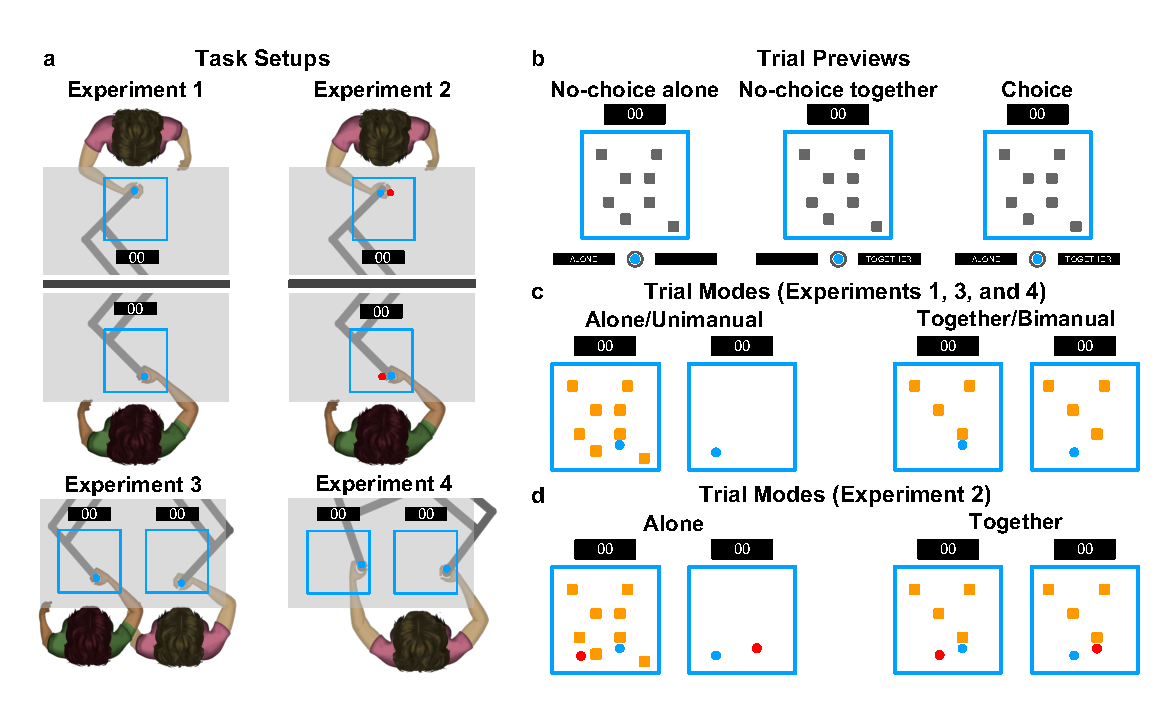
\includegraphics[width=1\linewidth,height=\textheight,keepaspectratio]{../../figures/fig1.pdf}

}

\subcaption{\label{fig-figure1}\emph{Note}. Participant pairs
(Experiments 1-3) performed a virtual ``box-clearing'' task in either
the Decision-maker role or the Helper role, or individually (Experiment
4) in either a unimanual or bimanual mode. Experimental setups differed
across experiments \textbf{(a)} but in all experiments, participants saw
a virtual cursor (blue circle) that represented their unseen hand, along
with individual workspaces (blue square) and a scoreboard. In
Experiments 1 and 2, each participant sat in front of a separate Kinarm
End-Point Lab that naturally positioned participants away (3.05 m) and
out of sight of one another. In Experiment 2, participants also received
online visual feedback of their partner's cursor location (red circle).
In Experiment 3, participant pairs were seated side-by-side in front of
a single, shared Kinarm End-Point Lab, and centered with their
respective workspace. In Experiments 1-3, the location of the
Decision-maker's workspace was counterbalanced across participants. In
Experiment 4, individual participants sat in front of a single Kinarm
End-Point lab, centered with the Primary workspace (counterbalanced
across participants). At the start of each trial, only the
Decision-maker was shown a preview of the target box arrangement for the
upcoming trial \textbf{(b)} and two task mode selection boxes. In the
no-choice trials, the Decision-maker was instructed to select the active
task mode selection box (i.e., only one contained text) by moving their
cursor into the box. In the choice trials, both task mode selection
boxes were active and the Decision-maker was instructed to choose one of
the two task modes. Once a task mode was selected, the selection boxes
disappeared and the target boxes changed colour from gray to orange
\textbf{(c-d)}. This change in colours served as the GO-signal for
participants. In alone (or unimanual) trials, all boxes shown in the
preview remained in the Decision-maker's (or Primary) workspace while
the Helper's (or Secondary) workspace remained empty. In together (or
bimanual) trials, the boxes were evenly distributed across each
workspace and appeared in the same arrangement. Trials ended once all
boxes were cleared or timed out after 100 s. One point per box was
earned for boxes cleared in the Decision-maker's (or Primary)
workspace.}

}

\end{figure}%

\clearpage

\subsection{Procedure}\label{procedure}

\subsubsection{Experiment 1: Separate Kinarm End-Point
Labs}\label{experiment-1-separate-kinarm-end-point-labs}

Participants pairs, which were created randomly, entered the lab and
were directed to sit at a desk to receive verbal and written
instructions about the experiment. Within each pair, participants were
randomly assigned as either the ``Decision-maker'' or the ``Helper''.
The Kinarm End-Point Lab occupied by the Decision-maker was
counterbalanced across participants. Each participant was seated in an
adjustable chair in front of an End-Point Lab at a height such that
their forehead could rest comfortably on the system's padded headrest.
The experimental setup naturally positioned the participants out of
sight from one another and at a distance of 3.05 m. Participants were
instructed that the task goal was for the Decision-maker to collect as
many points as possible by clearing boxes from their workspace (1 point
per box) within 30 mins. It was made clear that points were not earned
for any boxes cleared by the Helper on their respective workspace.
However, participants unknowingly completed a fixed number of trials,
which required less time to complete than this time limit. Participants
were also not permitted to communicate with one another throughout the
experiment.

In 50\% of trials, the Decision-maker was given the choice to perform
the task alone or with the Helper (choice trials). In the remaining 50\%
of trials, the Decision-maker was forced to do the task alone (no-choice
alone; 25\% of trials) or together (no-choice together; 25\% of trials).
The fixed number of no-choice alone and no-choice together trials were
included to ensure that each pair of participants experienced the same
minimum number of trials in each task mode, irrespective of the
Decision-maker's decisions in the choice trials. Within each task mode
(i.e., no-choice alone, no-choice together, and choice), we manipulated
the number of boxes that were displayed with either four, eight, or 12
boxes. All trial conditions were fully randomized and each number of
boxes appeared an equal number of times. All participants experienced
the same randomized order of trial and box conditions.

The experiment began with four familiarization trials (two no-choice
alone and two no-choice together), followed by 180 experimental trials
consisting of 90 choice, 45 no-choice alone, and 45 no-choice together
in a random order. Each trial began with a preview of the box
configuration for the upcoming trial displayed to the Decision-maker
(Figure~\ref{fig-figure1}B). Boxes were gray during the preview.
Participants then moved their virtual cursor into the home position.
After holding this position for 500 ms, two rectangles appeared at the
bottom of the display on opposite sides of the home position. In the
choice task mode, the word ALONE appeared in one rectangle and TOGETHER
in the other. The Decision-maker would move their cursor into one of the
two rectangles to select the task mode they wanted for the upcoming
trial. In the no-choice task mode, when the two rectangles appeared only
one contained text to indicate the task mode for the upcoming trial. The
Decision-maker would then move their virtual cursor into this rectangle.
The rectangle that the ALONE and TOGETHER text appeared in was
counterbalanced across pairs. Once the Decision-maker moved their cursor
into the selected (choice task mode) or the imposed (no-choice task
mode) rectangle, the boxes changed from gray to orange, signifying the
start of that trial. The trial ended once the last box was cleared or
after 100 s elapsed. On alone trials, boxes appeared only in the
Decision-maker's workspace and thus, could only be cleared by the
Decision-maker. On together trials, the boxes were evenly distributed
across each participant's workspace and appeared in the same arrangement
(Figure~\ref{fig-figure1}C). During these trials, both participants had
to ``hit'' boxes in the same grid location with their cursors, within a
pre-specified time window of \(\leq\) 200 ms. If they ``hit'' different
boxes or did not ``hit'' the same box within the synchrony threshold,
the box remained on the screen until synchronously hit. Participants had
no feedback of each other's movements and were not permitted to
communicate with each other. One point was awarded for every box cleared
from the Decision-maker's workspace. A box above the participant's
workspace showed the cumulative number of points earned and was updated
at the end of each trial. This design ensured that performing the task
together was not only suboptimal in terms of maximizing reward (i.e.,
points per trial), but also increased movement costs associated with
coordinating their actions (i.e., same box in \(\leq\) 200 ms) with
their partner.

After participants completed all experimental trials, the
Decision-makers were asked a series of open-ended questions regarding
their decision-making processes. The Decision-makers answered these
questions by typing their responses in a survey form on a laptop that
were saved for later analysis. Participants were asked to answer the
following questions: a) ``When given the choice to do the task alone or
together with the Helper, \emph{why} did you choose to complete the task
\emph{alone}?'', b) ``When given the choice to do the task alone or
together with the Helper, \emph{when} did you choose to complete the
task \emph{alone}?'', c) ``When given the choice to do the task alone or
together with the Helper, \emph{why} did you choose to complete the task
\emph{together}?'', d) ``When given the choice to do the task alone or
together with the Helper, \emph{when} did you choose to complete the
task \emph{together}?'', and e) ``Is there anything else you would like
to tell us about how you completed the task?''. No follow-up questions
were asked regarding participants' responses. Participants required
approximately five minutes to complete this part of the experiment.

\subsubsection{Experiment 2: Online Visual
Feedback}\label{experiment-2-online-visual-feedback}

The task, apparatus, and procedures matched Experiment 1, with two
exceptions. First, we provided online visual feedback of each other's
movements by displaying both participants' cursors on each workspace
(Figure~\ref{fig-figure1}D). Providing online visual feedback of both
virtual cursors was intended to reduce, but not eliminate, the
instrumental cost incurred while coordinating with a partner. This
allowed us to assess preferences for cooperation when the cost of
cooperation was reduced compared to that in Experiment 1. Second, the
Decision-makers did not complete the open-ended questionnaire.

\subsubsection{Experiment 3: Shared Kinarm End-Point
Lab}\label{experiment-3-shared-kinarm-end-point-lab}

The task, apparatus, and procedures matched Experiment 1, with the
exception that participants were seated beside one another and performed
the task on the same Kinarm End-Point Lab (Figure~\ref{fig-figure1}A).
Positioning participants next to one another was intended to heighten
social pressure to cooperate due to the close physical proximity between
partners. Each participant grasped the handle of their own robot
manipulandum and there was no physical barrier or occlusion between them
or their workspaces when using their respective robot manipulandum.
Participants were instructed to only look at their own workspace
directly in front of them.

\subsubsection{Experiment 4: Solo
Control}\label{experiment-4-solo-control}

The task, apparatus, and procedures matched Experiment 3, with two
exceptions. First, the task was completed individually. Participants sat
in front of a Kinarm End-Point Lab and grasped the handles of both robot
manipulandums (Figure~\ref{fig-figure1}A). The task was performed either
unimanually or bimanually, serving as a control to the non-coordinated
and coordinated task modes of the partner experiments but in a
non-social context. Second, the participants did not complete the
open-ended questionnaire.

\subsection{Data Analysis}\label{data-analysis}

Alpha was set to .05 for all statistical tests, which are described
below. Corrected degrees of freedom using the Greenhouse-Geisser method
are always reported when appropriate. Generalized eta squared
\((\eta_{G}^{2})\) is reported as an effect size for all omnibus tests.
Post-hoc comparisons were performed using the Holm-Bonferroni approach
to adjust for multiple comparisons. Statistical analyses were conducted
using R (Version 4.6.0, R Core Team, 2024) and the R-packages
\emph{afex} (Version 1.5.1, Singmann et al., 2024), \emph{easystats}
(Version 0.7.6, Lüdecke et al., 2022), \emph{emmeans} (Version 2.0.3,
Lenth, 2024), \emph{grateful} (Version 0.3.0, Rodriguez-Sanchez \&
Jackson, 2025), \emph{here} (Version 1.0.2, Müller, 2025), \emph{Hmisc}
(Version 5.2.5, Harrell Jr, 2025), \emph{kableExtra} (Version 1.4.0,
Zhu, 2024), \emph{patchwork} (Version 1.3.2, Pedersen, 2024),
\emph{rcompanion} (Version 2.5.2, Mangiafico, 2024), \emph{renv}
(Version 1.2.3, Ushey \& Wickham, 2024), and \emph{tidyverse} (Version
2.0.0, Wickham et al., 2019) were used in this project.

\subsubsection{Choice Data}\label{choice-data}

Our primary outcome variable was the proportion of trials in the choice
task mode where the Decision-makers selected to perform the task with
the Helper (Experiments 1-3) and bimanually rather than unimanually
(Experiment 4). We analyzed the proportion of together (Experiments 1-3)
and bimanual (Experiment 4) trials using a two-tailed Wilcoxon
signed-rank test against chance level. We performed an exploratory
analysis on the proportion of together (or bimanual) choices as a
function of box number using a one-way repeated measures ANOVA.

To gain insights into the thought processes of the Decision-makers when
choosing to perform the task alone or together, we conducted inductive
(Braun \& Clarke, 2006) and abductive (Thompson, 2022) thematic content
analyses in Experiments 1 and 3, respectively, to identify, analyze, and
report themes within the open-ended questionnaire data. The analyses
were conducted in a stepwise process. First, the primary coder (M.L.)
read through all participants' responses to the open-ended questions and
made initial notes of the content of the data. This allowed the coder to
become familiar with the data, specifically the depth and breadth of the
responses. Next, the coder systematically worked through the entire data
set, identifying segments of responses (i.e., sentences, phrases, or
individual words) that shared similar ideas or topics. While identifying
such segments, the coder generated labels (initial codes) for each
common idea or topic.

In the inductive thematic analysis of the responses from Experiment 1,
the coder then generated various levels of themes by considering how
different codes could be combined to support overarching themes. The
coder first consolidated the initial codes into initial themes. These
initial themes were further combined to form intermediate themes.
Finally, the intermediate themes were once more grouped into a final set
of higher order themes. The operational definition, an example of a
participant's response, and the number of responses for each higher
order theme can be found in Table~\ref{tbl-table1}.

\clearpage
\begingroup
\setstretch{1}

\begin{landscape}\begingroup\fontsize{10}{12}\selectfont

\begin{longtable}[l]{>{\raggedright\arraybackslash}p{3.75cm}>{\raggedright\arraybackslash}p{5cm}>{\raggedright\arraybackslash}p{3cm}>{\raggedright\arraybackslash}p{3cm}>{\raggedright\arraybackslash}p{6cm}}

\caption{\label{tbl-table1}The final five higher order themes from
Experiment 1, their operational definitions, the intermediate and
initial themes, and an example of a participant's response.}

\tabularnewline

\toprule
Final Theme & Definition & Intermediate Theme & Initial Theme & Example\\
\midrule
Chose actions with greater instrumental utility  & Made decisions with the intention of reducing the time or energy needed to complete the task, and/or increasing the amount of points that could be earned. & Reduced instrumental costs & Maximized speed & “I decided to do all the optional tasks alone because I knew it would be faster...” (Participant 212)\\
\addlinespace
 &  &  &  \vphantom{1} & \\
\addlinespace
 &  &  &  & \\
\addlinespace
 &  &  & Minimized movement & “I attempted to complete the task in the most effective and quickest way, moving the handle with the shortest distance possible.” (Participant 111)\\
\addlinespace
 &  & Reduced cognitive costs & Minimized decisions required & “I chose to do the task alone when there were many boxes that were far away from each other as I knew it would be difficult to choose the same boxes as the helper.” (Participant 101)\\
\addlinespace
 &  &  & Minimized difficult coordination & “[I chose alone] because it was more reliable and gave more points, it eliminated the variable of having to depend on another person’s timing and thinking.” (Participant 107)\\
\addlinespace
 &  & Minimized task constraints & Completed the task in the “easiest” way & “It was easier to complete the task alone” (Participant 404)\\
\addlinespace
 &  &  & Considered the spatial arrangement of the boxes & “[I chose together] when there was not as high of a concentration of squares, but also when they were in close proximity with each other.”\\
\addlinespace
 &  & Maximized instrumental rewards & NA & “I chose to complete the task alone when I realized that the number of points I got from working together was not as much as working alone.” (Participant 412)\\
\addlinespace
Chose actions with greater social value & Made decisions that were motivated by enhancing their own and/or their partner's experience. & Maximized intrinsic rewards & NA & “I found it more fun and interesting when I had to complete the task together because you can see how similarly or differently you and your partner think and what each person's first instinct is.” (Participant 312)\\
\addlinespace
 &  & Prosocial behaviour & Empathy & “[I chose together] because I felt bad for my partner if he was left with nothing to do” (Participant 102)\\
\addlinespace
 &  &  & Fairness & “I chose to do the task together when I had done a few trials alone. I thought that my partner would be upset if I did a bunch of the trials on my own just to achieve more points, so I would sometimes choose to do them with her to make it more fair. “ (Participant 410)\\
\addlinespace
Flexibility in decision strategy & Open to changing their decisions throughout the course of the experiment. & NA & NA & “There were some instances where I felt me and the helper changed the way we were slicing the squares to try to imitate each other...” (Participant 211)\\
\addlinespace
Planned movement path & Discussed their own individual directional patterns they typically moved in and/or the order they planned to clear boxes in. & NA & NA & “I noticed I tended to hit the boxes in a circular motion starting from the one closest to me, moving outwards, then returning to the starting area.” (Participant 309)\\
\addlinespace
Made reliable decisions & Made decisions knowing they could perform the task consistently well in that task mode. & NA & NA & “[I chose alone] because it was more reliable and gave more points, it eliminated the variable of having to depend on another person’s timing and thinking.” (Participant 107)\\
\bottomrule

\end{longtable}

\endgroup{}
\end{landscape}

\endgroup
\clearpage

The coding and identification of themes from the responses in Experiment
3 were guided by the coding framework generated in Experiment 1. This
abductive approach both bolsters and challenges the generalizability of
our current theoretical understanding, strengthening our confidence in
the existing theory while remaining responsive to surprising findings
(Timmermans \& Tavory, 2012). The coder engaged in a similar repetitive
consolidating process as described for Experiment 1, which resulted in
initial themes, intermediate themes, and a final set of higher order
themes. The operational definition, an example of a participant's
response, and the number of responses for each higher order theme can be
found in Table~\ref{tbl-table2}.

To ensure the validity of the identified themes and a reliable portrayal
of the data by the primary coder, intercoder reliability was measured
during the thematic analysis process following the guidelines of
O'Connor \& Joffe (2020). This process involved comparing the agreement
of coding between two coders. After grouping the initial codes into
final themes, the primary coder provided a comparison coder (J.T. in
Experiment 1 and M.M.C. in Experiment 3) with a random selection of 50\%
of the codes, as well as a list of the final themes and the respective
operational definitions. The comparison coder was instructed to sort
each code into one of the final themes to the best of their knowledge
using the theme names and definitions. A comparison analysis was
performed to determine intercoder reliability between coders, which
resulted in Cohen's \(\kappa\) of .88 and .81 for Experiments 1 and 3,
respectively. These values are larger than the recommended minimum value
of .80 (Hruschka et al., 2004), suggesting strong intercoder reliability
and confirming that the primary coder accurately represented the data
within the final themes.

\clearpage
\begingroup
\setstretch{1}

\begin{landscape}\begingroup\fontsize{10}{12}\selectfont

\begin{longtable}[l]{>{\raggedright\arraybackslash}p{3.75cm}>{\raggedright\arraybackslash}p{5cm}>{\raggedright\arraybackslash}p{3cm}>{\raggedright\arraybackslash}p{3cm}>{\raggedright\arraybackslash}p{6cm}}

\caption{\label{tbl-table2}The final six higher order themes from
Experiment 3, their operational definitions, the intermediate and
initial themes, and an example of a participant's response.}

\tabularnewline

\toprule
Final Theme & Definition & Intermediate Theme & Initial Theme & Example\\
\midrule
Chose actions with greater instrumental utility & Made decisions with the intention of reducing the time or energy needed to complete the task, and/or increasing the amount of points that could be earned. & Reduced instrumental costs & Maximized speed & “I chose to complete the task alone when I felt it would be quicker than doing it together.” (Participant 108)\\
\addlinespace
 &  &  & Prioritized efficiency & “Doing the task alone is more efficient and requires less effort…” (Participant 207)\\
\addlinespace
 &  & Reduced cognitive costs & Minimized cognitive strain & “[I chose alone] because it would be easier [to] do it on my own. Doing it together entails greater cognitive load.” (Participant 205)\\
\addlinespace
 &  &  & Minimized difficult coordination & “[I chose alone] when I thought it would be hard to coordinate to hit the dots at the same time” (Participant 105)\\
\addlinespace
 &  & Minimized task constraints & Completed the task in the “easiest” way & “I chose to do the task alone to eliminate the boxes faster as it was easier for me to do it alone.” (Participant 403)\\
\addlinespace
 &  &  & Considered the spatial arrangement of the boxes & “I would choose to complete the task alone when the boxes were seen as farther apart. When the boxes were closer together, I believed that it would be easier to complete the task together.” (Participant 208)\\
\addlinespace
 &  &  & Considered the number of boxes & “[I chose together’ when there wasn't many boxes on the screen.” (Participant 101)\\
\addlinespace
 &  & Maximized instrumental rewards & Maximized points & “I chose to do the task alone more often because it would give us higher points.” (Participant 311)\\
\addlinespace
Chose actions with greater social value & Made decisions that were motivated by enhancing their own and/or their partner's  experience. & Extrinsic motivations of prosocial behaviour & Reputation management & “I chose to do it together because I didn't want to seem rude for never choosing to do it together…” (Participant 210)\\
\addlinespace
 &  & Intrinsic motivations of prosocial behaviour & Cooperation was intrinsically rewarding & “I chose to do the task together because it was fun when we did it together…” (Participant 201)\\
\addlinespace
 &  &  & Empathy & “I usually didn't want the helper to feel left out and wanted to get them as many opportunities as possible” (Participant 407)\\
\addlinespace
 &  &  & Fairness & “When there were a lot of alone trials in a row sometimes I would switch it up to make it a together trial.” (Participants 401)\\
\addlinespace
Made informed decisions & Made decisions knowing they could perform the task consistently well in that task mode, sometimes influenced by performance in previous trials. & Made reliable decisions & NA & “I would choose to complete the task alone because at times I trusted my own judgment, methods, and coordination alone more than my partner's ability to synchronize with me.” (Participant 308)\\
\addlinespace
 &  & Previous performance informed decisions & NA & “I chose to do the tasks alone when I felt that the helper made a series of errors during previous runs.” (Participant 111)\\
\addlinespace
Considered partner dynamics & Conveyed their own or inferred their partner's intentionality through sensorimotor communication strategies or observed improved partner dynamics. & Learning opportunity & NA & “To practice, after a "together" task took a bit more time or led to some confusion between us.” (Participant 104)\\
\addlinespace
 &  & Improved partner dynamics & NA & “[I chose together] when I was able to understand what boxes he would move his cursor [to] first so I was able to get the hang of it and we were able to finish boxes together at a faster rate.” (Participant 410)\\
\addlinespace
Planned movement path & Discussed their own individual directional patterns they typically moved in and/or the order they planned to clear boxes in. & NA & NA & “Most tasks, I chose to do it from right to left (right-handed), or in proximity- closest to farthest.” (Participant 213)\\
\addlinespace
Developed a decision preference & Developed a preference to complete the task alone or together throughout the experiment. & NA & NA & “If there were a greater amount of boxes, I would choose to complete the task alone. Towards the end of the experiment, I would always choose to complete the task alone if the option was given.“ (Participant 207)\\
\bottomrule

\end{longtable}

\endgroup{}
\end{landscape}

\endgroup
\clearpage

\subsubsection{Box Clearing Data}\label{box-clearing-data}

Our second outcome variable was trial completion time for no-choice
trials, which was the interval of time between the boxes turning orange
and the last box being cleared. We analyzed mean trial time using a 2
Task Mode (Alone/Unimanual, Together/Bimanual) x 3 Number of Boxes (4,
8, 12) repeated measures ANOVA. We also analyzed distance traveled for
no-choice trials, which was the total distance that an individual's
cursor moved in the interval of time between the boxes turning orange
and the last box being cleared (see Supplementary 1).

\section{Results}\label{results}

\subsection{Experiment 1: Separate Kinarm End-Point
Labs}\label{experiment-1-separate-kinarm-end-point-labs-1}

Participants did not prefer to complete the task with their Helper on
free-choice trials and there was a downward trend in the proportion of
together choices as box number increased (Figure~\ref{fig-figure2}a).
The proportion of together choices was not significantly different from
chance level, \emph{V} = 472.5, \emph{p} = .112, \emph{r} = -.225
{[}-.478, .068{]}. Participants chose to perform the task together more
often when there were fewer boxes to clear, \emph{F}(1.51, 74.06) =
16.43, \emph{p} \textless{} .001, \(\eta_{G}^{2}\) = .057. The mean
proportion of together choices was greater for 4 boxes than 8 boxes
(\emph{p} = .001, \emph{d} = .42), for 4 boxes than 12 boxes (\emph{p}
\textless{} .001, \emph{d} = .57), and for 8 boxes than 12 boxes
(\emph{p} = .023, \emph{d} = .16).

\clearpage

\begin{figure}

\caption{\label{fig-figure2}The proportion of together/bimanual choices
on free-choice trials}

\centering{

\centering{

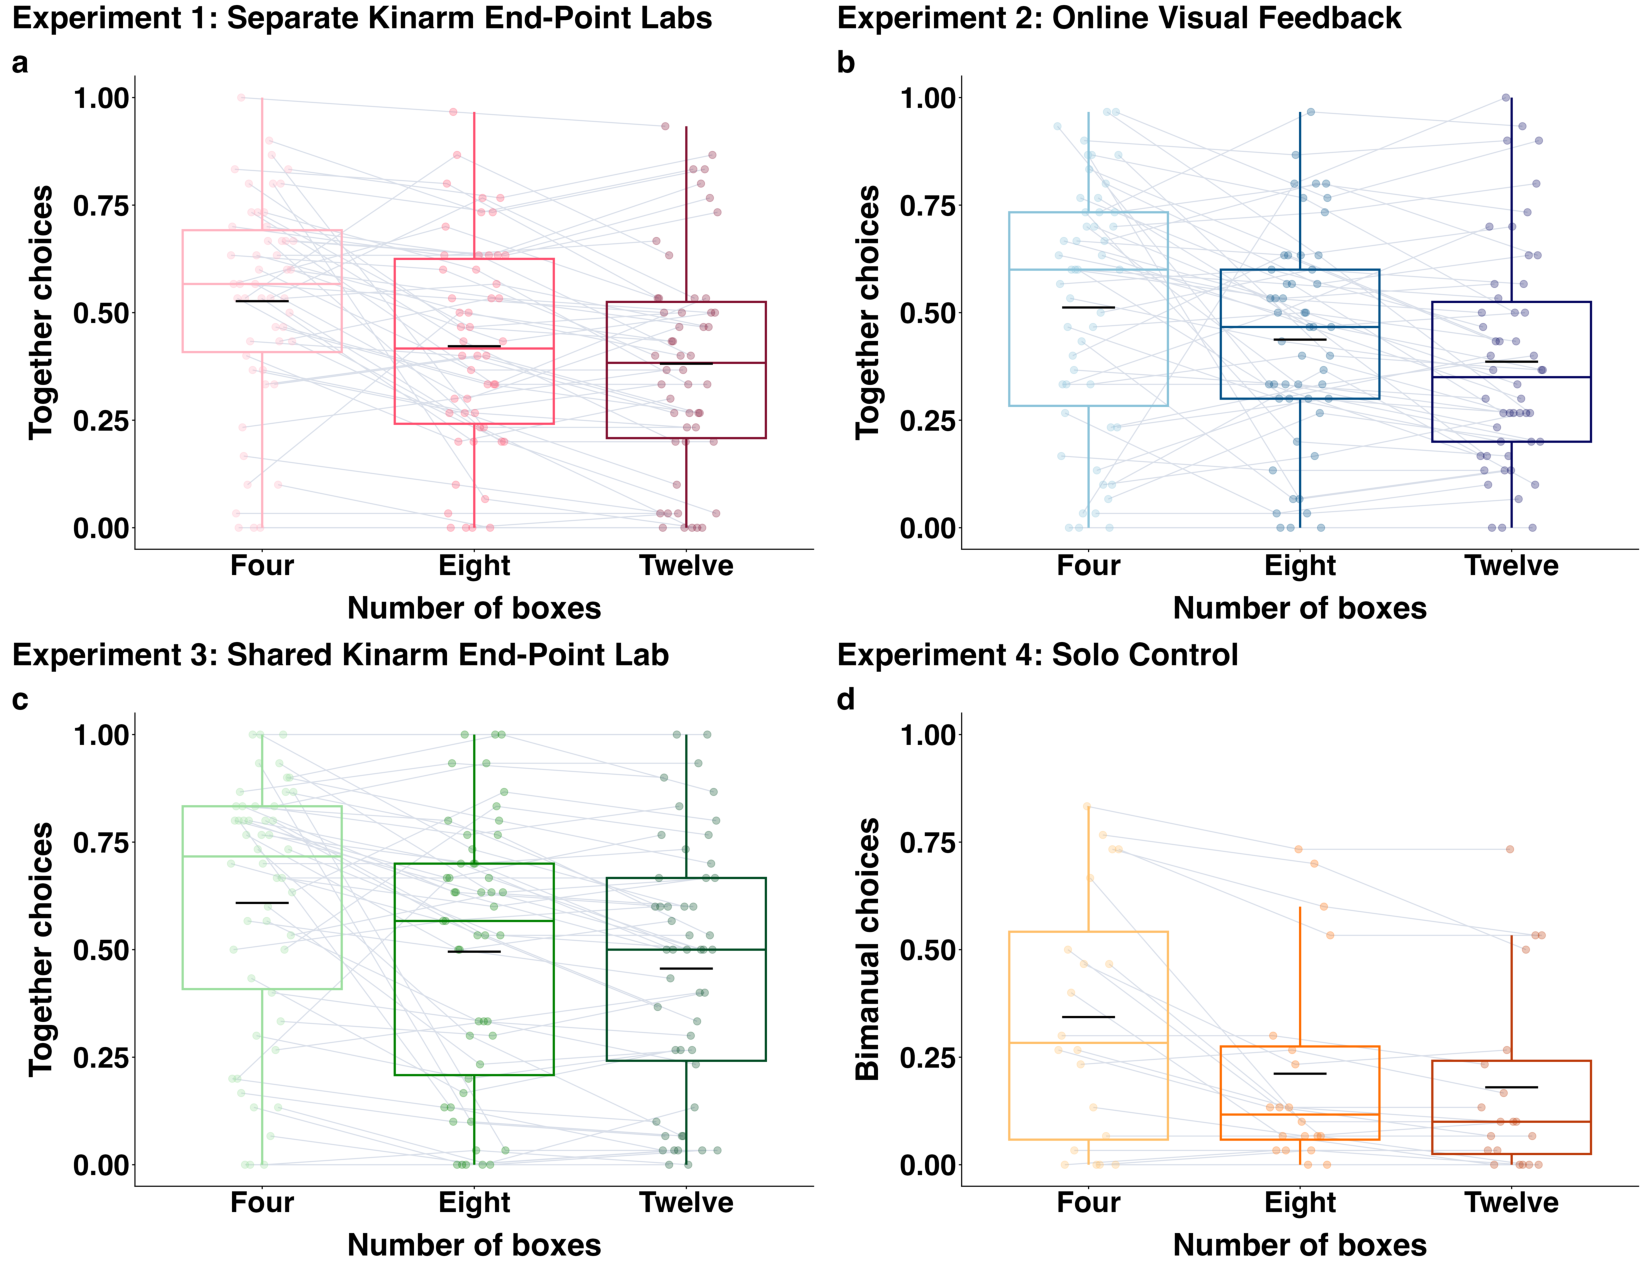
\includegraphics[width=1\linewidth,height=\textheight,keepaspectratio]{../../figures/fig2.pdf}

}

\subcaption{\label{fig-figure2}\emph{Note}. During the partner
experiments the Decision-maker could choose to perform the task either
alone or together with their Helper on 90 choice trials. During the solo
experiment the Decision-maker could choose to perform the task either
unimanually or bimanually. These choice trials were randomly interleaved
with the forced alone (unimanual) and forced together (bimanual) trials.
Boxplots of the proportion of together \textbf{(a-c)} and bimanual
\textbf{(d)} choices as a function of the number of boxes on choice
trials. Boxplots represent the 25th, 50th, and 75th percentiles, and the
solid black line denotes the mean. Individual dots connected by grey
lines represent means from individual participants.}

}

\end{figure}%

\clearpage

Five final themes were identified, which represented participants'
reasoning behind their decisions: a) chose actions with greater
instrumental utility, b) chose actions with greater social value, c)
made reliable decisions, d) flexibility in decision strategy, and e)
planned movement path. The two most prominent higher order themes were
each composed of several intermediate and initial themes. The
intermediate themes within the final theme ``chose actions with greater
instrumental utility'' reflect the separate cost and reward components
of instrumental utility, and highlight the complexity of the costs
associated with action alternatives. Intermediate themes within the
final theme ``chose actions with greater social value'' reflect efforts
to maximize intrinsic rewards and act prosocially, considering the
Helper's feelings or perspectives and choosing the task condition with
the intention of being inclusive to their partner.

Participants were faster (Figure~\ref{fig-figure3}a) at performing the
task alone (\emph{M} = 2.55 s, \emph{SD} = 0.52) compared to together
(\emph{M} = 4.82 s, \emph{SD} = 1.95). The significant main effects of
Task Mode, \emph{F}(1, 49) = 74.33, \emph{p} \textless{} .001,
\(\eta_{G}^{2}\) = .323, and Number of Boxes, \emph{F}(1.57, 76.85) =
266.51 \emph{p} \textless{} .001, \(\eta_{G}^{2}\) = .422, were
superseded by a significant Task Mode × Number of Boxes interaction,
\emph{F}(1.52, 74.57) = 56.57, \emph{p} \textless{} .001,
\(\eta_{G}^{2}\) = .130. Post hoc analyses revealed that participants
were significantly faster at performing the task alone than together
with 4 boxes (\emph{p} \textless{} .001, \emph{d} = .68), with 8 boxes
(\emph{p} \textless{} .001, \emph{d} = 1.54), and with 12 boxes
(\emph{p} \textless{} .001, \emph{d} = 1.56). Participants were also
significantly faster at performing the task with 4 boxes than 8 boxes
alone (\emph{p} \textless{} .001, \emph{d} = 1.47) and together
(\emph{p} \textless{} .001, \emph{d} = 1.44), as well as with 4 boxes
than 12 boxes alone (\emph{p} \textless.001, \emph{d} = 1.50) and
together (\emph{p} \textless{} .001, \emph{d} = 1.52), and with 8 boxes
than 12 boxes alone (\emph{p} \textless{} .001, \emph{d} = .85) and
together (\emph{p} \textless{} .001, \emph{d} = .79). The effect of task
mode and box number on distance traveled were in line with the findings
for trial time (see Supplementary 1).

\clearpage

\begin{figure}

\caption{\label{fig-figure3}The time required to clear boxes on forced
alone/unimanual and forced together/bimanual trials}

\centering{

\centering{

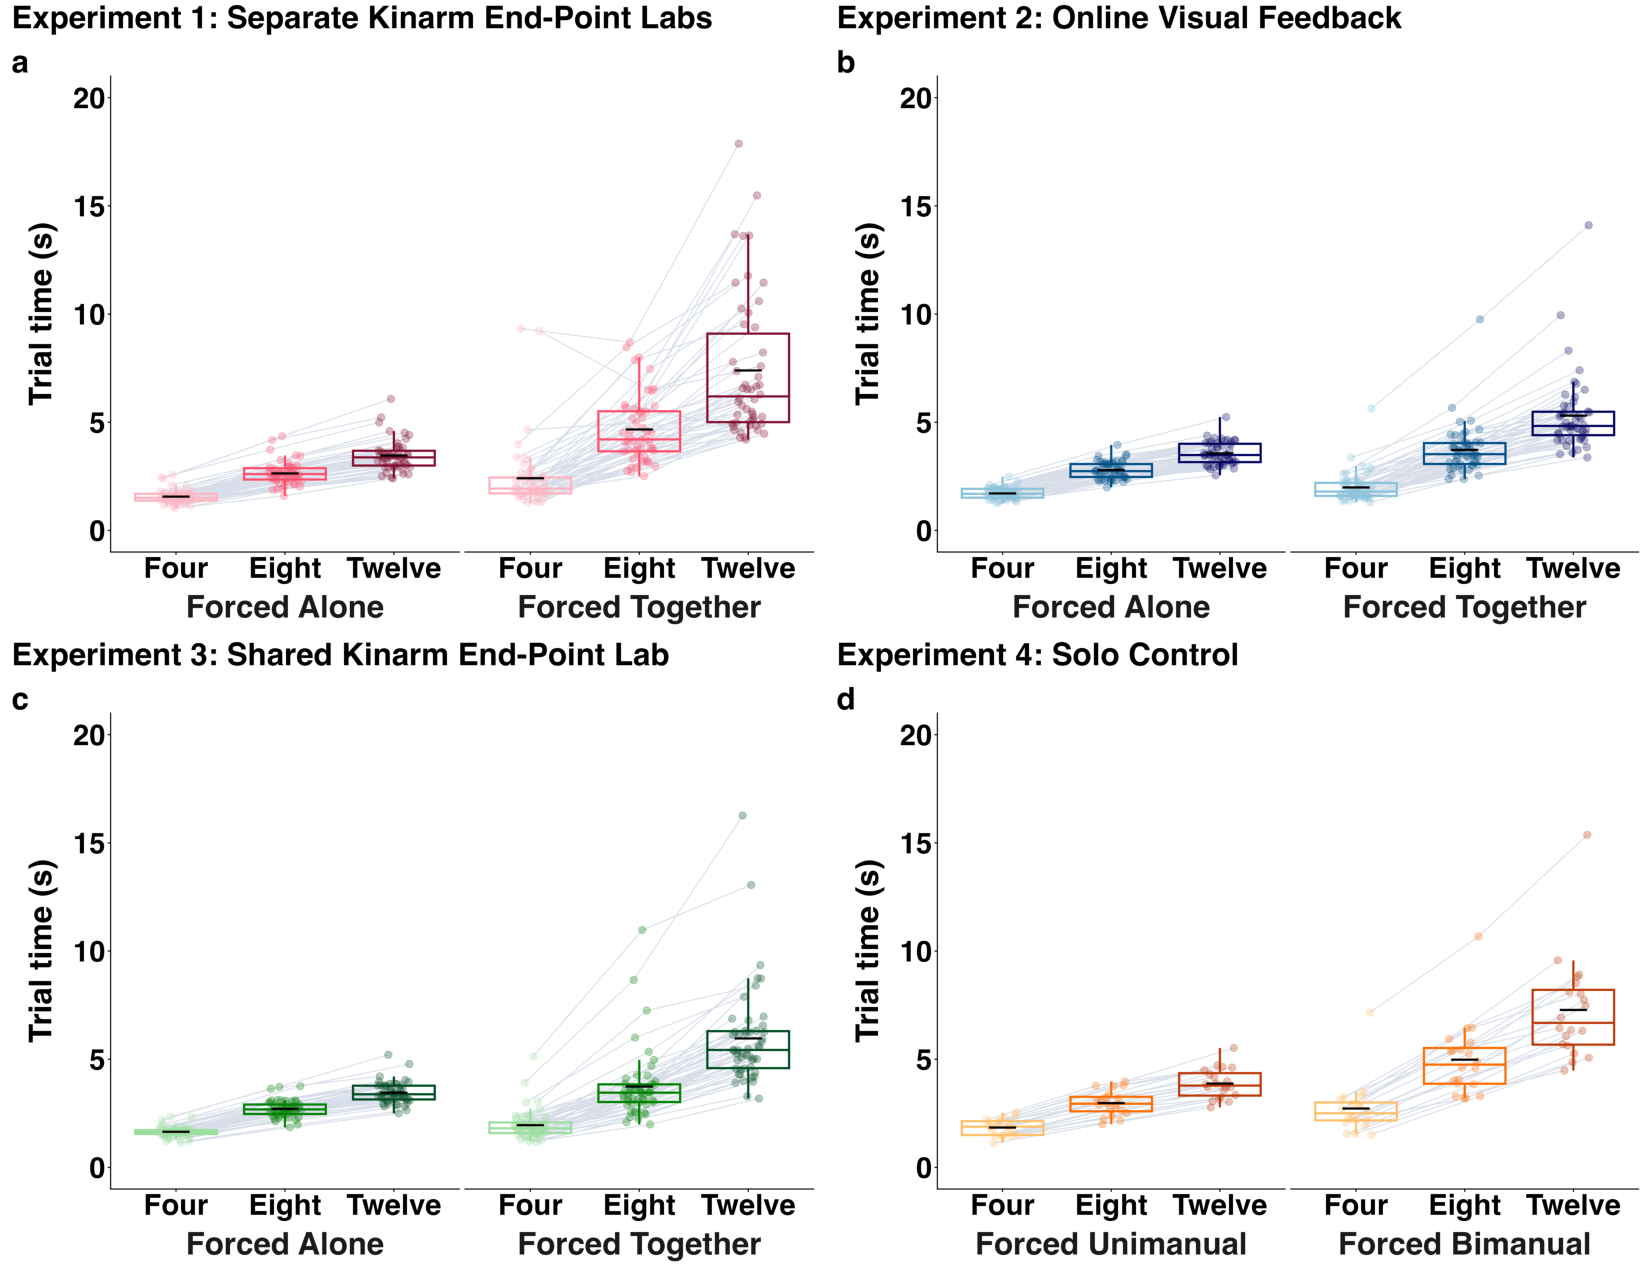
\includegraphics[width=1\linewidth,height=\textheight,keepaspectratio]{../../figures/fig3.pdf}

}

\subcaption{\label{fig-figure3}\emph{Note}. Boxplots of mean trial time
(s), which was the interval of time between the boxes turning orange and
the last box cleared, for each box condition in the forced alone and
forced together trials of the partner experiments \textbf{(a-c)} and the
forced unimanual and forced bimanual trials of the solo experiment
\textbf{(d)}. Boxplots represent the 25th, 50th, and 75th percentiles,
and the solid black line denotes the mean. Individual dots connected by
grey lines represent means from individual participants.}

}

\end{figure}%

\clearpage

\subsection{Experiment 2: Online Visual
Feedback}\label{experiment-2-online-visual-feedback-1}

Similar to Experiment 1, participants did not prefer to complete the
task with their Helper on free-choice trials and there was a downward
trend in the proportion of together choices as box number increased
(Figure~\ref{fig-figure2}b). The proportion of together choices was not
significantly different from chance level, \emph{V} = 493, \emph{p} =
.164, \emph{r} = -.198 {[}-.447, .065{]}. Participants chose to perform
the task together more often when there were fewer boxes to clear,
\emph{F}(1.28, 62.79) = 7.13, \emph{p} = .006, \(\eta_{G}^{2}\) = .037.
The mean proportion of together choices was greater for 4 boxes than 8
boxes (\emph{p} = .041, \emph{d} = .45), for 4 boxes than 12 boxes
(\emph{p} = .013, \emph{d} = .75), and for 8 boxes than 12 boxes
(\emph{p} = .014, \emph{d} = .33).

Participants were faster (Figure~\ref{fig-figure3}b) at performing the
task alone (\emph{M} = 2.68 s, \emph{SD} = 0.38) compared to together
(\emph{M} = 3.67 s, \emph{SD} = 1.16). The significant main effects of
Task Mode, \emph{F}(1, 49) = 44.44, \emph{p} \textless{} .001,
\(\eta_{G}^{2}\) = .218, and Number of Boxes, \emph{F}(1.28, 69.92) =
690.26 \emph{p} \textless{} .001, \(\eta_{G}^{2}\) = .561, were
superseded by a significant Task Mode × Number of Boxes interaction,
\emph{F}(1.25, 61.47) = 72.87, \emph{p} \textless{} .001,
\(\eta_{G}^{2}\) = .094. Post hoc analyses revealed that participants
were significantly faster at performing the task alone than together
with 4 boxes (\emph{p} = .005, \emph{d} = .46), with 8 boxes (\emph{p}
\textless{} .001, \emph{d} = .98), and with 12 boxes (\emph{p}
\textless{} .001, \emph{d} = 1.17). Participants were also significantly
faster at performing the task with 4 boxes than 8 boxes alone (\emph{p}
\textless{} .001, \emph{d} = 2.24) and together (\emph{p} \textless{}
.001, \emph{d} = 1.25), with 4 boxes than 12 boxes alone (\emph{p}
\textless{} .001, \emph{d} = 2.82) and together (\emph{p} \textless{}
.001, \emph{d} = 1.22), and with 8 boxes than 12 boxes alone (\emph{p}
\textless{} .001, \emph{d} = 1.37) and together (\emph{p} \textless{}
.001, \emph{d} = .75). The effect box number on distance traveled was in
line with the findings for trial time, while task mode had the opposite
effect (see Supplementary 1).

\subsection{Experiment 3: Shared Kinarm End-Point
Labs}\label{experiment-3-shared-kinarm-end-point-labs}

Participants had a preference to complete the task with their Helper on
free-choice trials and there was a downward trend in the proportion of
together choices as box number increased (Figure~\ref{fig-figure2}c).
The proportion of together choices was not significantly greater than
chance level, \emph{V} = 704, \emph{p} = .524, \emph{r} = .091 {[}-.171,
.376{]}. Participants chose to perform the task together more often when
there were fewer boxes to clear, \emph{F}(1.20, 58.89) = 13.92, \emph{p}
\textless{} .001, \(\eta_{G}^{2}\) = .045. The mean proportion of
together choices was greater for 4 boxes than 8 boxes (\emph{p} = .003,
\emph{d} = .37), for 4 boxes than 12 boxes (\emph{p} \textless{} .001,
\emph{d} = .51), and for 8 boxes than 12 boxes (\emph{p} = .006,
\emph{d} = .13).

Six final themes were identified, which represented participants'
reasoning behind their decisions: a) chose actions with greater
instrumental utility, b) chose actions with greater social value, c)
considered partner dynamics, d) made informed decisions, e) developed
decision preference, and f) planned movement path. The two most
prominent higher order themes were each composed of several intermediate
and initial themes. Within the final theme ``chose actions with greater
instrumental utility'', participants expressed desires to reduce
instrumental and cognitive costs, as well as task constraints. Within
the final theme ``chose actions with greater social value'',
participants reported intrinsic and extrinsic motivations for engaging
in prosocial behaviour. Intrinsic motivators aligned with general
feelings of intrinsic reward from cooperating while extrinsic motivation
came from the desire to manage their reputation. Intermediate themes
within the final theme ``made informed decisions'' indicate that
participants sought to make reliable decisions and used performance on
previous trials to inform subsequent decisions. Lastly, within the final
theme ``considered partner dynamics'', participants expressed
observations of or attempts to improve coordination dynamics with their
partner.

Participants were faster (Figure~\ref{fig-figure3}c) at performing the
task alone (\emph{M} = 2.60 s, \emph{SD} = 0.37) compared to together
(\emph{M} = 3.88 s, \emph{SD} = 1.46). The significant main effects of
Task Mode, \emph{F}(1, 49) = 46.83, \emph{p} \textless{} .001,
\(\eta_{G}^{2}\) = .225, and Number of Boxes, \emph{F}(1.26, 61.92) =
404.93 \emph{p} \textless{} .001, \(\eta_{G}^{2}\) = .500, were
superseded by a significant Task Mode × Number of Boxes interaction,
\emph{F}(1.31, 63.97) = 81.07, \emph{p} \textless{} .001,
\(\eta_{G}^{2}\) = .130. Post hoc analyses revealed that participants
were significantly faster at performing the task alone than together
with 4 boxes (\emph{p} = .003, \emph{d} = .54), with 8 boxes (\emph{p}
\textless{} .001, \emph{d} = .75), and with 12 boxes (\emph{p}
\textless{} .001, \emph{d} = 1.20). Participants were also significantly
faster at performing the task with 4 boxes than 8 boxes alone (\emph{p}
\textless{} .001, \emph{d} = 1.90) and together (\emph{p} \textless{}
.001, \emph{d} = .67), with 4 boxes than 12 boxes alone (\emph{p}
\textless{} .001, \emph{d} = 2.53) and together (\emph{p} \textless{}
.001, \emph{d} = 1.36), and with 8 boxes than 12 boxes alone (\emph{p}
\textless{} .001, \emph{d} = 1.42) and together (\emph{p} \textless{}
.001, \emph{d} = .92). The effect of task mode and box number on
distance traveled were in line with the findings for trial time (see
Supplementary 1).

\subsection{Experiment 4: Solo
Control}\label{experiment-4-solo-control-1}

Participants preferred to complete the task unimanually compared to
bimanually on free-choice trials and there was a downward trend in the
proportion of bimanual choices as box number increased
(Figure~\ref{fig-figure2}d). The proportion of bimanual choices was
significantly smaller than chance level, \emph{V} = 14, \emph{p}
\textless{} .001, \emph{r} = -.76 {[}-.87, -.543{]}. Participants chose
to perform the task bimanually more often when there were fewer boxes to
clear, \emph{F}(1.16, 21.97) = 14.69, \emph{p} \textless{} .001,
\(\eta_{G}^{2}\) = .077. The mean proportion of bimanual choices was
greater for 4 boxes than 8 boxes (\emph{p} = .005, \emph{d} = .48), for
4 boxes than 12 boxes (\emph{p} = .001, \emph{d} = .59), and for 8 boxes
than 12 boxes (\emph{p} = .018, \emph{d} = .13).

Participants were faster (Figure~\ref{fig-figure3}d) at performing the
task unimanually (\emph{M} = 2.90 s, \emph{SD} = 0.54) compared to
bimanually (\emph{M} = 4.99 s, \emph{SD} = 1.75). The significant main
effects of Task Mode, \emph{F}(1, 19) = 43.94, \emph{p} \textless{}
.001, \(\eta_{G}^{2}\) = .384, and Number of Boxes, \emph{F}(1.23,
23.42) = 302.96 \emph{p} \textless{} .001, \(\eta_{G}^{2}\) = .507, were
superseded by a significant Task Mode × Number of Boxes interaction,
\emph{F}(1.22, 23.16) = 78.91, \emph{p} \textless{} .001,
\(\eta_{G}^{2}\) = .131. Post hoc analyses revealed that participants
were significantly faster at performing the task unimanually than
bimanually with 4 boxes (\emph{p} = .002, \emph{d} = .73), with 8 boxes
(\emph{p} \textless{} .001, \emph{d} = 1.12), and with 12 boxes
(\emph{p} \textless{} .001, \emph{d} = 1.32). Participants were also
significantly faster at performing the task with 4 boxes than 8 boxes
unimanually (\emph{p} \textless{} .001, \emph{d} = 1.45) and bimanually
(\emph{p} \textless{} .001, \emph{d} = .95), with 4 boxes than 12 boxes
unimanually (\emph{p} \textless{} .001, \emph{d} = 2.04) and bimanually
(\emph{p} \textless{} .001, \emph{d} = 1.18), and with 8 boxes than 12
boxes unimanually (\emph{p} \textless{} .001, \emph{d} = 1.24) and
bimanually (\emph{p} \textless{} .001, \emph{d} = .75). The effect of
task mode and box number on distance traveled were in line with the
findings for trial time (see Supplementary 1).

\section{General Discussion}\label{general-discussion}

Our main finding across three partner experiments was that participants
did not significantly prefer costly joint action over completing the
same task alone, contrary to Curioni et al. (2022). Together choices
varied considerably at the individual level (range: 0-100\%), which was
reflected in the self-reported responses on the open-ended
questionnaires. Although Experiments 1 and 2 showed a small,
non-significant preference for solo action that was less than what would
be predicted by principles of utility and optimization (Jara-Ettinger et
al., 2016; Jara-Ettinger et al., 2020; Shadmehr et al., 2016; Todorov,
2004), participants in Experiment 4 (i.e., solo control) strongly
preferred completing the task unimanually, suggesting a sensitivity to
action costs in their decisions. Taken together, and in line with
Curioni et al. (2022), our behavioral and questionnaire data suggest
that humans assign additional reward value to performing actions with
others.

In our partner experiments, had participants only considered the
instrumental costs and rewards of the action alternatives as in the
Naive Utility Calculus (Jara-Ettinger et al., 2016; Jara-Ettinger et
al., 2020), one would expect to see participants predominantly select
the less costly action (i.e., solo) on free-choice trials. As such, it
was surprising to see that the proportion of together choices hovered
around 50\% in these experiments. Yet, removing the social context
(Experiment 4) led participants to behave more optimally, suggesting
that social factors are considered as part of the calculus when faced
with an action alternative involving joint action. Indeed, our
participants described working together as being intrinsically rewarding
and that they felt motivated by the enjoyment and enrichment they
experienced from the added challenge of coordinating as captured in our
higher order theme ``chose actions with greater social value''.
Participants also acknowledged prosocial behaviors (Eisenberg et al.,
2015) influencing their decision processes when choosing to perform the
task with their Helper (e.g., Michael et al., 2020; Obhi \& Sebanz,
2011; {van der Wel et al.}, 2021). These individuals empathized with the
Helper, choosing together when they felt bad that their partner was left
doing nothing or had not participated in a while. This resulted in some
participants balancing the distribution of alone and together trials
throughout the experiment as a way to be fair towards their partner.
Such deliberate behavior likely contributed to why the average
proportion of together choices did not differ from chance.
Interestingly, non-human primates are also sensitive to prosociality
(Brocard et al., 2025); however, cooperation appears to be largely
reward-driven, with decisions to cooperate typically occurring under
favorable payoff conditions (Quarta et al., 2025). This suggests that
while non-human primates can perceive prosocial behavior, cooperation
consistently motivated by such behavior may be more characteristic of
humans. Accordingly, if an additional, generic reward value is assigned
to performing a task with another person, decisions may depend strongly
on the individual and/or socio-cultural factors, which may be a fruitful
avenue for future studies.

Although social factors influenced the decision to cooperate---such that
some participants almost always chose to perform the task with their
Helper---others appeared more sensitive to the costs of joint action,
with a subset rarely or never including their Helper. This was
reinforced in participants' responses as they explicitly acknowledged
the additional costs and reduced instrumental benefits of joint action,
captured in the higher order theme ``chose actions with greater
instrumental utility''. Decision-makers reported being mindful of the
task goal (i.e., earn as many points as possible) and often preferred to
complete the task in the mode they believed would be fastest and/or
require the fewest movements, which was overwhelmingly perceived to be
the solo condition. Along these lines, participants described choosing
to work together when fewer boxes needed to be cleared, as a larger
number of boxes increased the difficulty of repeatedly selecting the
same box and coordinating their movements. Given this, it is not
surprising that we found that participants made significantly less
together choices as the number of boxes to clear increased (see
Figure~\ref{fig-figure2}). The ability to predict a partner's behavior
is an important mechanism for successful joint action (Sebanz et al.,
2006) as seen by the reduction in trial time and distance traveled when
online visual feedback was provided (Experiment 1 vs 2 in
Figure~\ref{fig-figure3}). While this feedback likely facilitated
monitoring individual and joint outcomes (Bekkering et al., 2009; Loehr
et al., 2013), it may have also permitted the emergence of
``leader-follower'' dynamics (Candidi et al., 2015; Sacheli et al.,
2013) or allowed participants to rely on action-based communication
(Pezzulo et al., 2013; Pezzulo et al., 2019) to better convey their
intentions and resolve task uncertainty (e.g., Vesper \& Richardson,
2014; Vesper et al., 2016). Despite reducing coordination costs, online
visual feedback did not result in a higher proportion of together
trials; thus, future research should explore these mechanisms within the
context of costly cooperation.

We did not observe a significant preference for costly joint action in
our experiments, despite its robustness in Curioni et al. (2022),
suggesting that this effect may depend on task or participant
characteristics. One possibility is that our version of the task,
reaching to boxes in a virtual environment, was more costly than their
version, tapping boxes in the real-world. This seems likely given that
trial times in our partner experiments for both the solo (2.55, 2.68,
and 2.60 s) and together (4.82, 3.67, 3.88 s) trials were much slower
compared to those in Curioni and colleagues (2022) for both solo (1.58
s) and together (1.80 s) trials. This is consistent with past research
demonstrating that target-based movements in virtual environments are
slower and less accurate than the same movements in the real-world
(Arnold et al., 2002; {Liu et al.}, 2009). Thus, our heightened
coordination demands may have simply outweighed any intrinsic reward
value assigned to cooperation, irrespective of the physical proximity of
participants. A future experiment could resolve this by having
participants perform the ``box-clearing'' task on separate touchscreen
tablets.

A possible limitation of our experiment is our use of a convenience
sample, meaning some participant pairs may have already been familiar
with one another compared to others, or complete strangers. Partners
also briefly interacted with one another upon entering the lab and
received experimental instructions together. These brief social
interactions, such as greeting (Sandstrom, 2023) and making eye contact
(Wesselmann et al., 2012) could have elicited feelings of social
connectedness. While it may be beneficial in future research to control
these factors, we argue that it was more ecologically valid to allow
these brief moments of interaction to occur. Similar to Curioni et al.
(2022), our participant pairs were created randomly without controlling
for sex, gender, age, or ethnicity. Demographics and identification with
co-actors have been shown to impact decisions to cooperate (e.g., Chuah
et al., 2014; Chen et al., 2012; Krumhuber et al., 2007; Levy et al.,
2004), ability to coordinate (Boukarras et al., 2021), and partner
choice in interactive tasks (Chuah et al., 2014; Krumhuber et al.,
2007). Exploring the influence of these factors in future research may
have important practical implications, especially in workplace settings.

In conclusion, despite not finding a strong preference for costly joint
action, the proportion of choosing to perform the task alone were much
lower than would be expected if these decisions were solely guided by
principles of optimization and utility, as seen when decisions were made
in a non-social context. Our behavioral and questionnaire data add
further support to the idea that additional rewards are derived from the
social nature of joint action (e.g., Curioni et al., 2022) and that
these preferences are highly individualized.

\clearpage

\section{References}\label{references}

\protect\phantomsection\label{refs}
\begin{CSLReferences}{1}{0}
\bibitem[\citeproctext]{ref-arnold2002}
Arnold, P., Farrell, M. J., Pettifer, S., \& West, A. J. (2002).
Performance of a skilled motor task in virtual and real environments.
\emph{Ergonomics}, \emph{45}(5), 348--361.
\url{https://doi.org/10.1080/00140130110120510}

\bibitem[\citeproctext]{ref-bekkering2009}
Bekkering, H., De Bruijn, E. R. A., Cuijpers, R. H., Newman-Norlund, R.,
Van Schie, H. T., \& Meulenbroek, R. (2009). Joint {Action}:
{Neurocognitive Mechanisms Supporting Human Interaction}. \emph{Topics
in Cognitive Science}, \emph{1}(2), 340--352.
\url{https://doi.org/10.1111/j.1756-8765.2009.01023.x}

\bibitem[\citeproctext]{ref-boukarras2021}
Boukarras, S., Era, V., Aglioti, S. M., \& Candidi, M. (2021).
Competence-based social status and implicit preference modulate the
ability to coordinate during a joint grasping task. \emph{Scientific
Reports}, \emph{11}(1), 5321.
\url{https://doi.org/10.1038/s41598-021-84280-z}

\bibitem[\citeproctext]{ref-braun2006}
Braun, V., \& Clarke, V. (2006). Using thematic analysis in psychology.
\emph{Qualitative Research in Psychology}, \emph{3}(2), 77--101.

\bibitem[\citeproctext]{ref-brocard2025}
Brocard, S., Berton, C., Wilson, V., Bickel, B., \& Zuberbühler, K.
(2025). The perception of prosocial agents by chimpanzees and humans.
\emph{Royal Society Open Science}, \emph{12}(11), 250916.
\url{https://doi.org/10.1098/rsos.250916}

\bibitem[\citeproctext]{ref-calalo2025}
Calalo, J. A., Ngo, T. T., Sullivan, S. R., Strand, K., Buggeln, J. H.,
Lokesh, R., Roth, A. M., Carter, M. J., Kurtzer, I. L., \& Cashaback, J.
G. (2025). Online movements reflect ongoing deliberation. \emph{Journal
of Neuroscience}, \emph{45}(31).

\bibitem[\citeproctext]{ref-candidi2015}
Candidi, M., Curioni, A., Donnarumma, F., Sacheli, L. M., \& Pezzulo, G.
(2015). Interactional leader--follower sensorimotor communication
strategies during repetitive joint actions. \emph{Journal of The Royal
Society Interface}, \emph{12}(110), 20150644.
\url{https://doi.org/10.1098/rsif.2015.0644}

\bibitem[\citeproctext]{ref-chen2012}
Chen, J., Zhong, J., Zhang, Y., Li, P., Zhang, A., Tan, Q., \& Li, H.
(2012). Electrophysiological correlates of processing facial
attractiveness and its influence on cooperative behavior.
\emph{Neuroscience Letters}, \emph{517}(2), 65--70.
\url{https://doi.org/10.1016/j.neulet.2012.02.082}

\bibitem[\citeproctext]{ref-chuah2014}
Chuah, S.-H., Hoffmann, R., Ramasamy, B., \& Tan, J. H. (2014).
Religion, ethnicity and cooperation: {An} experimental study.
\emph{Journal of Economic Psychology}, \emph{45}, 33--43.

\bibitem[\citeproctext]{ref-cos2011}
Cos, I., Bélanger, N., \& Cisek, P. (2011). The influence of predicted
arm biomechanics on decision making. \emph{Journal of Neurophysiology},
\emph{105}(6), 3022--3033. \url{https://doi.org/10.1152/jn.00975.2010}

\bibitem[\citeproctext]{ref-cos2014}
Cos, I., Duque, J., \& Cisek, P. (2014). Rapid prediction of
biomechanical costs during action decisions. \emph{Journal of
Neurophysiology}, \emph{112}(6), 1256--1266.
\url{https://doi.org/10.1152/jn.00147.2014}

\bibitem[\citeproctext]{ref-curioni2022}
Curioni, A., Voinov, P., Allritz, M., Wolf, T., Call, J., \& Knoblich,
G. (2022). Human adults prefer to cooperate even when it is costly.
\emph{Proceedings of the Royal Society B: Biological Sciences},
\emph{289}(1973), 20220128. \url{https://doi.org/10.1098/rspb.2022.0128}

\bibitem[\citeproctext]{ref-eisenberg2015}
Eisenberg, N., Eggum, N. D., \& Spinrad, T. L. (2015). {114The
Development} of {Prosocial Behavior}. In D. A. Schroeder \& W. G.
Graziano (Eds.), \emph{The {Oxford Handbook} of {Prosocial Behavior}}
(p. 0). Oxford University Press.
\url{https://doi.org/10.1093/oxfordhb/9780195399813.013.008}

\bibitem[\citeproctext]{ref-gallivan2018}
Gallivan, J. P., Chapman, C. S., Wolpert, D. M., \& Flanagan, J. R.
(2018). Decision-making in sensorimotor control. \emph{Nature Reviews
Neuroscience}, \emph{19}(9), 519--534.
\url{https://doi.org/10.1038/s41583-018-0045-9}

\bibitem[\citeproctext]{ref-gordon2021}
Gordon, J., Maselli, A., Lancia, G. L., Thiery, T., Cisek, P., \&
Pezzulo, G. (2021). The road towards understanding embodied decisions.
\emph{Neuroscience \& Biobehavioral Reviews}, \emph{131}, 722--736.
\url{https://doi.org/10.1016/j.neubiorev.2021.09.034}

\bibitem[\citeproctext]{ref-harrell2025}
Harrell Jr, F. E. (2025). \emph{Hmisc: {Harrell} miscellaneous}
{[}Manual{]}.

\bibitem[\citeproctext]{ref-hruschka2004}
Hruschka, D. J., Schwartz, D., St.John, D. C., Picone-Decaro, E.,
Jenkins, R. A., \& Carey, J. W. (2004). Reliability in {Coding
Open-Ended Data}: {Lessons Learned} from {HIV Behavioral Research}.
\emph{Field Methods}, \emph{16}(3), 307--331.
\url{https://doi.org/10.1177/1525822X04266540}

\bibitem[\citeproctext]{ref-jara-ettinger2016}
Jara-Ettinger, J., Gweon, H., Schulz, L. E., \& Tenenbaum, J. B. (2016).
The {Naïve Utility Calculus}: {Computational Principles Underlying
Commonsense Psychology}. \emph{Trends in Cognitive Sciences},
\emph{20}(8), 589--604. \url{https://doi.org/10.1016/j.tics.2016.05.011}

\bibitem[\citeproctext]{ref-jara-ettinger2020}
Jara-Ettinger, J., Schulz, L. E., \& Tenenbaum, J. B. (2020). The {Naïve
Utility Calculus} as a unified, quantitative framework for action
understanding. \emph{Cognitive Psychology}, \emph{123}, 101334.
\url{https://doi.org/10.1016/j.cogpsych.2020.101334}

\bibitem[\citeproctext]{ref-kahneman2012}
Kahneman, D., \& Tversky, A. (2012). Prospect {Theory}: {An Analysis} of
{Decision Under Risk}. In \emph{Handbook of the {Fundamentals} of
{Financial Decision Making}: Volume 4} (pp. 99--127). WORLD SCIENTIFIC.
\url{https://doi.org/10.1142/9789814417358_0006}

\bibitem[\citeproctext]{ref-knoblich2011}
Knoblich, G., Butterfill, S., \& Sebanz, N. (2011). Psychological
research on joint action: Theory and data. \emph{Psychology of Learning
and Motivation}, \emph{54}, 59--101.

\bibitem[\citeproctext]{ref-kourtis2014}
Kourtis, D., Knoblich, G., Woźniak, M., \& Sebanz, N. (2014). Attention
{Allocation} and {Task Representation} during {Joint Action Planning}.
\emph{Journal of Cognitive Neuroscience}, \emph{26}(10), 2275--2286.
\url{https://doi.org/10.1162/jocn_a_00634}

\bibitem[\citeproctext]{ref-krumhuber2007}
Krumhuber, E., Manstead, A. S., Cosker, D., Marshall, D., Rosin, P. L.,
\& Kappas, A. (2007). Facial dynamics as indicators of trustworthiness
and cooperative behavior. \emph{Emotion}, \emph{7}(4), 730.

\bibitem[\citeproctext]{ref-lenth2024}
Lenth, R. V. (2024). \emph{Emmeans: {Estimated} marginal means, aka
least-squares means} {[}Manual{]}.

\bibitem[\citeproctext]{ref-levy2004}
Levy, I., Kaplan, A., \& Patrick, H. (2004). Early {Adolescents}'
{Achievement Goals}, {Social Status}, and {Attitudes Towards
Cooperation} with {Peers}. \emph{Social Psychology of Education},
\emph{7}(2), 127--159.
\url{https://doi.org/10.1023/B:SPOE.0000018547.08294.b6}

\bibitem[\citeproctext]{ref-liu2009}
{Liu, L., van Liere, R., Nieuwenhuizen, C., \& Martens, J.-B.} (2009).
Comparing aimed movements in the real world and in virtual reality.
\emph{2009 {IEEE} Virtual Reality Conference}, 219--222.
\url{https://doi.org/10.1109/VR.2009.4811026}

\bibitem[\citeproctext]{ref-loehr2013}
Loehr, J. D., Kourtis, D., Vesper, C., Sebanz, N., \& Knoblich, G.
(2013). Monitoring individual and joint action outcomes in duet music
performance. \emph{Journal of Cognitive Neuroscience}, \emph{25}(7),
1049--1061.

\bibitem[\citeproctext]{ref-ludecke2022}
Lüdecke, D., Ben-Shachar, M. S., Patil, I., Wiernik, B. M., Bacher, E.,
Thériault, R., \& Makowski, D. (2022). Easystats: {Framework} for easy
statistical modeling, visualization, and reporting. \emph{CRAN}.
\url{https://doi.org/10.32614/CRAN.package.easystats}

\bibitem[\citeproctext]{ref-mangiafico2024}
Mangiafico, S. S. (2024). \emph{{rcompanion}: {Functions} to support
extension education program evaluation} {[}Manual{]}. Rutgers
Cooperative Extension.

\bibitem[\citeproctext]{ref-michael2020}
Michael, J., McEllin, L., \& Felber, A. (2020). Prosocial effects of
coordination -- {What}, how and why? \emph{Acta Psychologica},
\emph{207}, 103083. \url{https://doi.org/10.1016/j.actpsy.2020.103083}

\bibitem[\citeproctext]{ref-michael2016}
Michael, J., Sebanz, N., \& Knoblich, G. (2016a). Observing joint
action: {Coordination} creates commitment. \emph{Cognition}, \emph{157},
106--113. \url{https://doi.org/10.1016/j.cognition.2016.08.024}

\bibitem[\citeproctext]{ref-michael2016a}
Michael, J., Sebanz, N., \& Knoblich, G. (2016b). The {Sense} of
{Commitment}: {A Minimal Approach}. \emph{Frontiers in Psychology},
\emph{6}.

\bibitem[\citeproctext]{ref-moskowitz2023}
Moskowitz, J. B., Berger, S. A., Fooken, J., Castelhano, M. S.,
Gallivan, J. P., \& Flanagan, J. R. (2023). The influence of
movement-related costs when searching to act and acting to search.
\emph{Journal of Neurophysiology}, \emph{129}(1), 115--130.
\url{https://doi.org/10.1152/jn.00305.2022}

\bibitem[\citeproctext]{ref-mosteller1951}
Mosteller, F., \& Nogee, P. (1951). An {Experimental Measurement} of
{Utility}. \emph{Journal of Political Economy}, \emph{59}(5), 371--404.
\url{https://www.jstor.org/stable/1825254}

\bibitem[\citeproctext]{ref-muller2025}
Müller, K. (2025). \emph{Here: A simpler way to find your files}
{[}Manual{]}.

\bibitem[\citeproctext]{ref-nowak2005}
Nowak, M. A., \& Sigmund, K. (2005). Evolution of indirect reciprocity.
\emph{Nature}, \emph{437}(7063), 1291--1298.
\url{https://doi.org/10.1038/nature04131}

\bibitem[\citeproctext]{ref-oconnor2020}
O'Connor, C., \& Joffe, H. (2020). Intercoder {Reliability} in
{Qualitative Research}: {Debates} and {Practical Guidelines}.
\emph{International Journal of Qualitative Methods}, \emph{19},
1609406919899220. \url{https://doi.org/10.1177/1609406919899220}

\bibitem[\citeproctext]{ref-obhi2011}
Obhi, S. S., \& Sebanz, N. (2011). Moving together: Toward understanding
the mechanisms of joint action. \emph{Experimental Brain Research},
\emph{211}(3), 329--336. \url{https://doi.org/10.1007/s00221-011-2721-0}

\bibitem[\citeproctext]{ref-pedersen2024}
Pedersen, T. L. (2024). \emph{Patchwork: {The} composer of plots}
{[}Manual{]}.

\bibitem[\citeproctext]{ref-pezzulo2013}
Pezzulo, G., Donnarumma, F., \& Dindo, H. (2013). Human {Sensorimotor
Communication}: {A Theory} of {Signaling} in {Online Social
Interactions}. \emph{PLOS ONE}, \emph{8}(11), e79876.
\url{https://doi.org/10.1371/journal.pone.0079876}

\bibitem[\citeproctext]{ref-pezzulo2019}
Pezzulo, G., Donnarumma, F., Dindo, H., D'Ausilio, A., Konvalinka, I.,
\& Castelfranchi, C. (2019). The body talks: {Sensorimotor}
communication and its brain and kinematic signatures. \emph{Physics of
Life Reviews}, \emph{28}, 1--21.
\url{https://doi.org/10.1016/j.plrev.2018.06.014}

\bibitem[\citeproctext]{ref-quarta2025}
Quarta, E., Lacal, I., Grasso, S., Schito, A., Papagni, V., \&
Battaglia-Mayer, A. (2025). {COSTS AND BENEFITS OF ACTING TOGETHER}: {A
NON-HUMAN PRIMATE MODEL OF COOPERATIVE DECISION-MAKING}. \emph{bioRxiv},
2025.11.20.689048. \url{https://doi.org/10.1101/2025.11.20.689048}

\bibitem[\citeproctext]{ref-rcoreteam2024}
R Core Team. (2024). \emph{R: A language and environment for statistical
computing} {[}Manual{]}. R Foundation for Statistical Computing.

\bibitem[\citeproctext]{ref-rangel2008}
Rangel, A., Camerer, C., \& Montague, P. R. (2008). A framework for
studying the neurobiology of value-based decision making. \emph{Nature
Reviews Neuroscience}, \emph{9}(7), 545--556.
\url{https://doi.org/10.1038/nrn2357}

\bibitem[\citeproctext]{ref-rodriguez-sanchez2025}
Rodriguez-Sanchez, F., \& Jackson, C. P. (2025). \emph{Grateful:
{Facilitate} citation of {R} packages} {[}Manual{]}.

\bibitem[\citeproctext]{ref-sacheli2013}
Sacheli, L. M., Tidoni, E., Pavone, E. F., Aglioti, S. M., \& Candidi,
M. (2013). Kinematics fingerprints of leader and follower role-taking
during cooperative joint actions. \emph{Experimental Brain Research},
\emph{226}(4), 473--486.

\bibitem[\citeproctext]{ref-sandstrom2023}
Sandstrom, G. M. (2023). Even minimal student-instructor interactions
may increase enjoyment in the classroom: {Preliminary} evidence that
greeting your students may have benefits even if you can't remember
their names. \emph{Plos One}, \emph{18}(8), e0288166.

\bibitem[\citeproctext]{ref-schmidt2008}
Schmidt, R. C., \& Richardson, M. J. (2008). Dynamics of interpersonal
coordination. \emph{Coordination: Neural, Behavioral and Social
Dynamics}, 281--308.

\bibitem[\citeproctext]{ref-sebanz2006}
Sebanz, N., Bekkering, H., \& Knoblich, G. (2006). Joint action: Bodies
and minds moving together. \emph{Trends in Cognitive Sciences},
\emph{10}(2), 70--76. \url{https://doi.org/10.1016/j.tics.2005.12.009}

\bibitem[\citeproctext]{ref-sebanz2021}
Sebanz, N., \& Knoblich, G. (2021). Progress in {Joint-Action Research}.
\emph{Current Directions in Psychological Science}, \emph{30}(2),
138--143. \url{https://doi.org/10.1177/0963721420984425}

\bibitem[\citeproctext]{ref-shadmehr2016}
Shadmehr, R., Huang, H. J., \& Ahmed, A. A. (2016). A {Representation}
of {Effort} in {Decision-Making} and {Motor Control}. \emph{Current
Biology}, \emph{26}(14), 1929--1934.
\url{https://doi.org/10.1016/j.cub.2016.05.065}

\bibitem[\citeproctext]{ref-simmons2012}
Simmons, J. P., Nelson, L. D., \& Simonsohn, U. (2012). A 21 word
solution. \emph{Available at SSRN 2160588}.

\bibitem[\citeproctext]{ref-simonsohn2015}
Simonsohn, U. (2015). Small {Telescopes}: {Detectability} and the
{Evaluation} of {Replication Results}. \emph{Psychological Science},
\emph{26}(5), 559--569. \url{https://doi.org/10.1177/0956797614567341}

\bibitem[\citeproctext]{ref-singmann2024}
Singmann, H., Bolker, B., Westfall, J., Aust, F., \& Ben-Shachar, M. S.
(2024). \emph{Afex: {Analysis} of factorial experiments} {[}Manual{]}.

\bibitem[\citeproctext]{ref-sullivan2026}
Sullivan, S. R., Buggeln, J. H., Calalo, J. A., Ngo, T. T., Semrau, J.
A., Carter, M. J., \& Cashaback, J. G. (2026). \emph{Involuntary
feedback responses reflect a representation of partner actions}.
\url{https://doi.org/10.7554/elife.109734.1}

\bibitem[\citeproctext]{ref-thompson2022}
Thompson, J. (2022). A {Guide} to {Abductive Thematic Analysis}.
\emph{The Qualitative Report}.
\url{https://doi.org/10.46743/2160-3715/2022.5340}

\bibitem[\citeproctext]{ref-timmermans2012}
Timmermans, S., \& Tavory, I. (2012). Theory {Construction} in
{Qualitative Research}: {From Grounded Theory} to {Abductive Analysis}.
\emph{Sociological Theory}, \emph{30}(3), 167--186.
\url{https://doi.org/10.1177/0735275112457914}

\bibitem[\citeproctext]{ref-todorov2004}
Todorov, E. (2004). Optimality principles in sensorimotor control.
\emph{Nature Neuroscience}, \emph{7}(9), 907--915.
\url{https://doi.org/10.1038/nn1309}

\bibitem[\citeproctext]{ref-ushey2024}
Ushey, K., \& Wickham, H. (2024). \emph{Renv: {Project} environments}
{[}Manual{]}.

\bibitem[\citeproctext]{ref-vanderwel2021}
{van der Wel, R. P. R. D., Becchio, C., Curioni, A., \& Wolf, T.}
(2021). Understanding joint action: {Current} theoretical and empirical
approaches. \emph{Acta Psychologica}, \emph{215}, 103285.
\url{https://doi.org/10.1016/j.actpsy.2021.103285}

\bibitem[\citeproctext]{ref-vesper2014}
Vesper, C., \& Richardson, M. J. (2014). Strategic communication and
behavioral coupling in asymmetric joint action. \emph{Experimental Brain
Research}, \emph{232}(9), 2945--2956.

\bibitem[\citeproctext]{ref-vesper2016}
Vesper, C., Schmitz, L., Safra, L., Sebanz, N., \& Knoblich, G. (2016).
The role of shared visual information for joint action coordination.
\emph{Cognition}, \emph{153}, 118--123.
\url{https://doi.org/10.1016/j.cognition.2016.05.002}

\bibitem[\citeproctext]{ref-wesselmann2012}
Wesselmann, E. D., Cardoso, F. D., Slater, S., \& Williams, K. D.
(2012). To be looked at as though air: {Civil} attention matters.
\emph{Psychological Science}, \emph{23}(2), 166--168.

\bibitem[\citeproctext]{ref-wickham2019}
Wickham, H., Averick, M., Bryan, J., Chang, W., McGowan, L. D.,
François, R., Grolemund, G., Hayes, A., Henry, L., Hester, J., Kuhn, M.,
Pedersen, T. L., Miller, E., Bache, S. M., Müller, K., Ooms, J.,
Robinson, D., Seidel, D. P., Spinu, V., \ldots{} Yutani, H. (2019).
Welcome to the {tidyverse}. \emph{Journal of Open Source Software},
\emph{4}(43), 1686. \url{https://doi.org/10.21105/joss.01686}

\bibitem[\citeproctext]{ref-zhu2024}
Zhu, H. (2024). \emph{kableExtra: Construct complex table with 'kable'
and pipe syntax}. \url{https://doi.org/10.32614/CRAN.package.kableExtra}

\end{CSLReferences}

\clearpage
\setcounter{page}{1}
\resetlinenumber

\renewcommand{\thefigure}{S\arabic{figure}}
\setcounter{figure}{1}

\section{Supplementary 1}\label{supplementary-1}

\subsection{Distance Traveled}\label{distance-traveled}

\subsubsection{Experiment 1: Separate Kinarm End-Point
Labs}\label{experiment-1-separate-kinarm-end-point-labs-2}

Participants traveled a shorter distance (Figure~\ref{fig-figureS1}a)
alone (\emph{M} = 0.64 m, \emph{SD} = 0.05) compared to together
(\emph{M} = 0.93, \emph{SD} = 0.27). The significant main effects of
Task Mode, \emph{F}(1, 49) = 58.13, \emph{p} \textless{} .001,
\(\eta_{G}^{2}\) = .255, and Number of Boxes, \emph{F}(1.31, 64.22) =
370.88 \emph{p} \textless{} .001, \(\eta_{G}^{2}\) = .577, were
superseded by a significant Task Mode × Number of Boxes interaction,
\emph{F}(1.30, 63.69) = 62.23, \emph{p} \textless{} .001,
\(\eta_{G}^{2}\) = .173. Post hoc comparisons revealed that participants
traveled a significantly shorter distance when performing the task alone
than together with 8 boxes (\emph{p} \textless{} .001, \emph{d} = 1.26)
and with 12 boxes (\emph{p} \textless{} .001, \emph{d} = 1.38), but
there was no difference when performing the task alone or together with
4 boxes (\emph{p} = .247, \emph{d} = .19). Participants also traveled a
significantly shorter distance with 4 boxes than 8 boxes alone (\emph{p}
\textless{} .001, \emph{d} = 4.67) and together (\emph{p} \textless{}
.001, \emph{d} = 2.14), with 4 boxes than 12 boxes alone (\emph{p}
\textless{} .001, \emph{d} = 5.27) and together (\emph{p} \textless{}
.001, \emph{d} = 1.56), and with 8 boxes than 12 boxes alone (\emph{p}
\textless{} .001, \emph{d} = 2.20) and together (\emph{p} \textless{}
.001, \emph{d} = .88).

\subsubsection{Experiment 2: Online Visual
Feedback}\label{experiment-2-online-visual-feedback-2}

Participants traveled a shorter distance (Figure~\ref{fig-figureS1}b)
together (\emph{M} = 0.62 m, \emph{SD} = 0.05) compared to alone
(\emph{M} = 0.57, \emph{SD} = 0.14). The significant main effects of
Task Mode, \emph{F}(1, 49) = 8.32, \emph{p} = .006, \(\eta_{G}^{2}\) =
.046, and Number of Boxes, \emph{F}(1.27, 62.41) = 894.65 \emph{p}
\textless{} .001, \(\eta_{G}^{2}\) = .719, were superseded by a
significant Task Mode × Number of Boxes interaction, \emph{F}(1.33,
65.08) = 10.37, \emph{p} \textless{} .001, \(\eta_{G}^{2}\) = .021. Post
hoc comparisons revealed that participants traveled a significantly
longer distance when performing the task alone than together with 4
boxes (\emph{p} \textless{} .001, \emph{d} = -.165), but there was no
difference when performing the task alone or together with 8 boxes
(\emph{p} = .071, \emph{d} = -.37) or 12 boxes (\emph{p} = .60, \emph{d}
= -.09). Participants traveled a significantly shorter distance with 4
boxes than 8 boxes alone (\emph{p} \textless{} .001, \emph{d} = 5.32)
and together (\emph{p} \textless{} .001, \emph{d} = 1.97), with 4 boxes
than 12 boxes alone (\emph{p} \textless{} .001, \emph{d} = 4.86) and
together (\emph{p} \textless{} .001, \emph{d} = 1.74), and with 8 boxes
than 12 boxes alone (\emph{p} \textless{} .001, \emph{d} = 1.90) and
together (\emph{p} \textless{} .001, \emph{d} = .77).

\subsubsection{Experiment 3: Shared Kinarm End-Point
Lab}\label{experiment-3-shared-kinarm-end-point-lab-1}

Participants traveled a shorter distance (Figure~\ref{fig-figureS1}c)
alone (\emph{M} = 0.61 m, \emph{SD} = 0.04) compared to together
(\emph{M} = 0.66, \emph{SD} = 0.12). The significant main effects of
Task Mode, \emph{F}(1, 49) = 10.22, \emph{p} = .002, \(\eta_{G}^{2}\) =
.046 and Number of Boxes, \emph{F}(1.49, 73.24) = 934.59 \emph{p}
\textless{} .001, \(\eta_{G}^{2}\) = .790, were superseded by a
significant Task Mode × Number of Boxes interaction, \emph{F}(1.59,
77.98) = 94.38, \emph{p} \textless{} .001, \(\eta_{G}^{2}\) = .188. Post
hoc comparisons revealed that participants traveled a significantly
longer distance when performing the task alone than together with 4
boxes (\emph{p} \textless{} .001, \emph{d} = -1.55) and a significantly
shorter distance with 12 boxes (\emph{p} \textless{} .001, \emph{d} =
1.20), but there was no difference when performing the task alone or
together with 8 boxes (\emph{p} = .172, \emph{d} = .20). Participants
also traveled a significantly shorter distance with 4 boxes than 8 boxes
alone (\emph{p} \textless{} .001, \emph{d} = 6.15) and together
(\emph{p} \textless{} .001, \emph{d} = 2.04), with 4 boxes than 12 boxes
alone (\emph{p} \textless{} .001, \emph{d} = 5.87) and together
(\emph{p} \textless{} .001, \emph{d} = 3.54), and with 8 boxes than 12
boxes alone (\emph{p} \textless{} .001, \emph{d} = 2.22) and together
(\emph{p} \textless{} .001, \emph{d} = 1.71).

\clearpage

\begin{figure}

\caption{\label{fig-figureS1}The distance traveled while clearing all
boxes on forced alone/unimanual and forced together/bimanual trials}

\centering{

\centering{

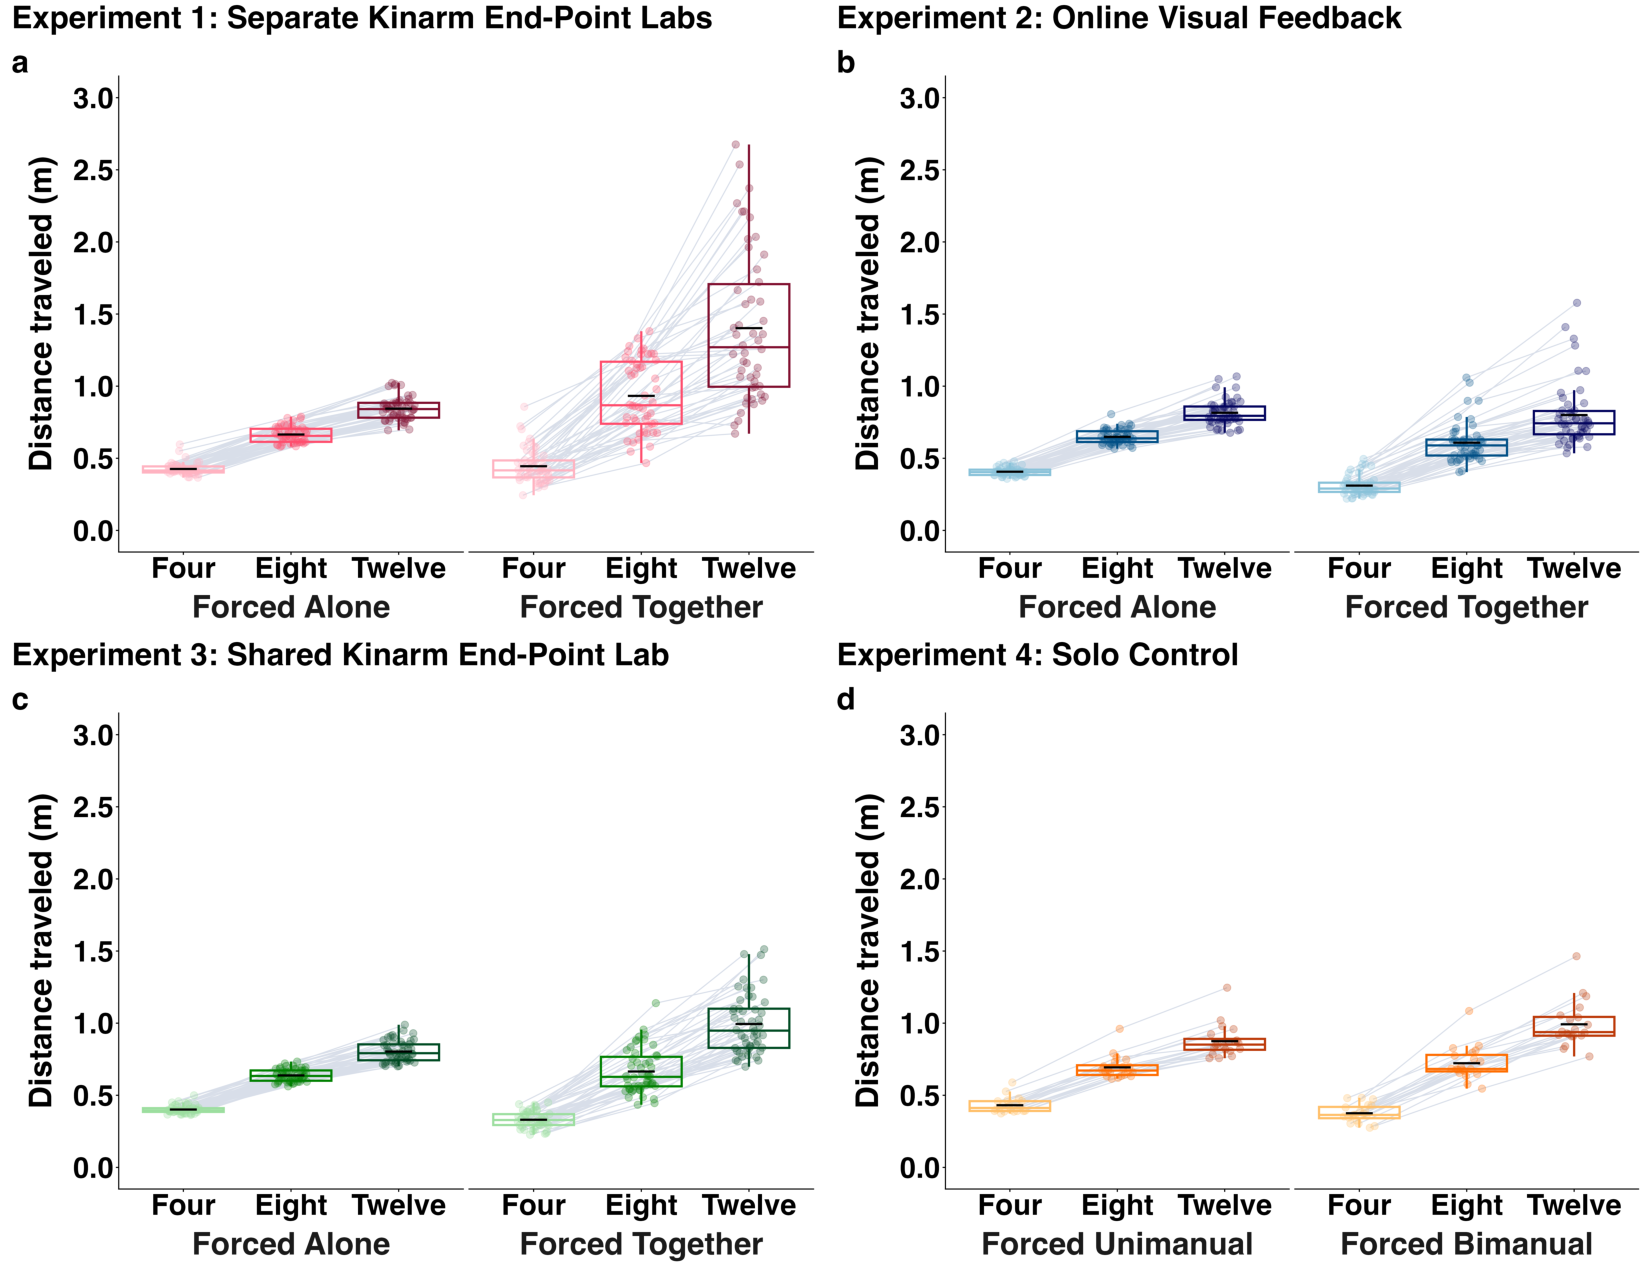
\includegraphics[width=1\linewidth,height=\textheight,keepaspectratio]{../../figures/figS1.pdf}

}

\subcaption{\label{fig-figureS1}\emph{Note}. Boxplots of mean distance
traveled (m), which was the total distance that a participant's cursor
moved during the interval of time between the boxes turning orange and
the last box cleared, for each box condition in the forced alone and
forced together trials of the partner experiments \textbf{(a-c)} and the
forced unimanual and forced bimanual trials of the solo experiment
\textbf{(d)}. Boxplots represent the 25th, 50th, and 75th percentiles,
and the solid black line denotes the mean. Individual dots connected by
grey lines represent means from individual participants.}

}

\end{figure}%

\clearpage

\subsubsection{Experiment 4: Solo
Control}\label{experiment-4-solo-control-2}

Participants traveled a slightly shorter distance
(Figure~\ref{fig-figureS1}d) unimanually (\emph{M} = 0.67 m, \emph{SD} =
0.08) compared to bimanually (\emph{M} = 0.70, \emph{SD} = 0.10). While
the main effect of Task Mode was not significant, \emph{F}(1, 19) =
3.22, \emph{p} = .089, \(\eta_{G}^{2}\) = .046, a main effect of Number
of Boxes, \emph{F}(1.39, 26.50) = 585.62 \emph{p} \textless{} .001,
\(\eta_{G}^{2}\) = .823, was superseded by a significant Task Mode ×
Number of Boxes interaction, \emph{F}(1.66, 31.56) = 46.59, \emph{p}
\textless{} .001, \(\eta_{G}^{2}\) = .109. Post hoc comparisons revealed
that participants traveled a significantly longer distance when
performing the task unimanually than bimanually with 4 boxes (\emph{p} =
.002, \emph{d} = -.95), and a significantly shorter distance with 12
boxes (\emph{p} \textless{} .001, \emph{d} = .80), but there was no
difference when performing the task unimanually or bimanually with 8
boxes (\emph{p} = .156, \emph{d} = .27). Participants also traveled a
significantly shorter distance with 4 boxes than 8 boxes unimanually
(\emph{p} \textless{} .001, \emph{d} = 3.14) and bimanually (\emph{p}
\textless{} .001, \emph{d} = 3.08), with 4 boxes than 12 boxes
unimanually (\emph{p} \textless{} .001, \emph{d} = 3.48) and bimanually
(\emph{p} \textless{} .001, \emph{d} = 3.64), and with 8 boxes than 12
boxes unimanually (\emph{p} \textless{} .001, \emph{d} = 1.56) and
bimanually (\emph{p} \textless{} .001, \emph{d} = 1.71).




\end{document}
